\documentclass[11pt,a4paper]{article}

% ---------------------------------------------------------------------------
% swig: exact joint placement of V, D and J for germline assignment.
% Build: latexmk -pdf main.tex   (see README.md for provenance of every number)
% ---------------------------------------------------------------------------

\usepackage[T1]{fontenc}
\usepackage[utf8]{inputenc}
\usepackage{lmodern}
\usepackage[margin=2.5cm]{geometry}
\usepackage{microtype}
\usepackage{amsmath,amssymb,amsthm}
\usepackage{mathtools}
\usepackage{booktabs}
\usepackage{multirow}
\usepackage{tabularx}
\usepackage{array}
\usepackage[table]{xcolor}
\usepackage{graphicx}
\usepackage{caption}
\usepackage{subcaption}
\usepackage{siunitx}
\sisetup{group-separator={,},group-minimum-digits=4,detect-weight=true,mode=text}
\usepackage{algorithm}
\usepackage{algpseudocode}
\usepackage{tikz}
\usetikzlibrary{arrows.meta,positioning,calc,fit,backgrounds,decorations.pathreplacing,shapes.misc}
\usepackage{pgfplots}
\usepgfplotslibrary{groupplots}
\pgfplotsset{compat=1.18}
\usepackage[numbers,sort&compress]{natbib}
\usepackage[colorlinks=true,linkcolor=blue!50!black,citecolor=blue!50!black,urlcolor=blue!50!black]{hyperref}
\usepackage[capitalise,noabbrev]{cleveref}

\newtheorem{lemma}{Lemma}
\newtheorem{theorem}{Theorem}
\theoremstyle{definition}
\newtheorem{definition}{Definition}

\newcommand{\swig}{\textsf{swig}}
\newcommand{\code}[1]{\texttt{#1}}
\newcommand{\pD}{P^{*}_{D}}
\newcommand{\phat}{\hat{p}}
\newcommand{\nats}{\,\text{nats}}
\newcommand{\pp}{\,pp}
\DeclareMathOperator*{\argmax}{arg\,max}

% Palette (colour-blind safe, after Okabe & Ito)
\definecolor{cV}{HTML}{0072B2}
\definecolor{cD}{HTML}{D55E00}
\definecolor{cJ}{HTML}{009E73}
\definecolor{cC}{HTML}{CC79A7}
\definecolor{cN}{HTML}{999999}
\definecolor{cSwig}{HTML}{0072B2}
\definecolor{cIgb}{HTML}{E69F00}
\definecolor{cMix}{HTML}{009E73}
\definecolor{cMixTop}{HTML}{56B4E9}
\definecolor{cOff}{HTML}{CC79A7}

\title{\swig: exact joint placement of V, D and J segments\\
for immune receptor germline assignment}

\author{Mateusz Kaduk\thanks{Affiliation to be added.}%
% TODO: co-authors and affiliations (the code is copyright MurrellGroup, MIT licence).
}

\date{Draft for swig 0.39.7 --- \today}

\begin{document}
\maketitle

% ===========================================================================
\begin{abstract}
\noindent\textbf{Motivation.}
Assigning germline V, D and J alleles and segment boundaries to adaptive immune
receptor reads is the first step of repertoire analysis, and everything
downstream inherits its errors. The D segment is short and trimmed at both
ends, somatic hypermutation blurs the evidence that separates alleles, and a
junction base that matches two segments can belong to either. Most aligners
place the segments one after another and accept a D by a tuned score
threshold.

\noindent\textbf{Results.}
We present \swig, a dependency-free Rust aligner that scores every segment
hypothesis as a log-likelihood ratio and chooses the alleles and the cut
points of V, D and J jointly, by an exact semi-Markov Viterbi recursion over a
placement graph. The recursion considers every pair of cuts between
neighbouring segments in time linear in their overlaps, and is checked
against exhaustive enumeration. The prior cost of each segment is derived as
prior odds over the gene-and-position hypotheses it competes with, rather
than tuned. A D also pays
geometric trim and N/P-length priors, and, at an open read end, the
likelihood ratio of the flanking segment the read would have shown. Each read
is valued at its own divergence, and forward--backward over the same graph
gives posterior probabilities of which the call is a mode. Seeded, banded
alignment over gene frames, lossless sibling bounds and an inter-sequence SIMD
Gotoh kernel make the search fast. On reads simulated by GenAIRR and scored
against its ambiguity-aware truth, \swig{} 0.39.7 has the highest V, D and J
accuracy of \swig{}, IgBLAST 1.22 and MiXCR 3.0.13 on every human
immunoglobulin set, raising human IGH D accuracy over IgBLAST by
0.7--6.0 percentage points across 0--10\,\% SHM (0.9--6.3 on reads disjoint
from those its D priors were designed on), and assigns about 7,000 reads per
second on four threads, 76--88 times the throughput of IgBLAST.

\noindent\textbf{Availability.}
\swig{} is open source under the MIT licence at
\url{https://github.com/mashu/swig} (crate \code{engine/}); it builds with
Rust $\geq 1.89$, has no dependencies, and compiles to native code and to
WebAssembly.
\end{abstract}

% ===========================================================================
\section{Introduction}

High-throughput sequencing of B- and T-cell receptor repertoires (AIRR-seq)
turns millions of rearranged receptor transcripts into reads. Each read is a
mosaic: a V, a D (heavy chains and TRB/TRD only) and a J gene segment, trimmed
by exonucleases at the joints and separated by non-templated N and
palindromic P nucleotides, and, in B cells, overlaid with somatic
hypermutation (SHM). Germline assignment names the allele of each segment and
locates its boundaries, which fixes the junction (CDR3). Clonal grouping,
mutation analysis, lineage reconstruction and inference of novel alleles all
start from these calls, so their errors propagate.

Three properties make the assignment uncertain rather than merely
expensive. First, human IGHD genes are 11--37 nucleotides long and lose
several bases at each end; a remnant of 4--8 nucleotides is common, and
random sequence matches a few bases of some D gene by chance at many
junction positions. Second, under SHM a mismatch may be a mutation, a
sequencing error or the base that separates two alleles. Third, an N base
that happens to match the neighbouring germline can be explained by either
segment, so where V ends, where D starts and where J starts are decided
together. The task is therefore to choose the most probable explanation
among many partial ones, and to say how probable it is.

Widely used tools approach it in different ways. IgBLAST~\cite{ye2013igblast}
and IMGT/V-QUEST~\cite{brochet2008vquest} align the read to V germlines and
then search for D and J in the remaining sequence. MiXCR~\cite{bolotin2015mixcr}
uses $k$-mer seeding and alignment for speed. partis~\cite{ralph2016partis}
annotates with hidden Markov models whose parameters are inferred from the
repertoire, at a much higher computational cost. Benchmarks with an
ambiguity-aware simulator~\cite{konstantinovsky2024genairr} show that these
aligners make distinct errors, most of them in D. Deciding segments in
sequence lets a neighbour's local alignment absorb a short D, and fixed
score thresholds for accepting a D trade sensitivity on short remnants
against spurious D calls on D-free junctions in ways that are hard to
interpret.

\swig{} instead defines one objective, a log-likelihood ratio over the whole
read, and maximises it exactly over the segment alleles and every pair of cut
points between neighbouring segments. Its contributions are:
\begin{enumerate}
  \item a \emph{placement graph} over candidate V, D and J alignments whose
    semi-Markov Viterbi recursion is exact over all grammatical paths and all
    cut pairs, in time linear in the overlaps between placements
    (\cref{sec:dag});
  \item segment priors \emph{derived} as prior odds over the hypotheses
    a segment competes with,
    D trim and N/P-length priors that re-rank D alleles without changing
    how often a typical D is called, and an \emph{open-flank} cost for a D at
    a truncated read end (\cref{sec:objective});
  \item calls valued at each read's own divergence in exact integer
    arithmetic, with forward--backward posteriors over the same graph, so
    the call is a mode of the reported distribution (\cref{sec:perread,sec:posterior});
  \item a search whose every shortcut is labelled with its guarantee (exact,
    lossless, bounded, defined, approximate or heuristic), including lossless
    sibling bounds over gene frames
    (\cref{sec:search}), and an inter-sequence SIMD kernel that is
    bit-identical to a scalar Gotoh across x86-64, AArch64 and WebAssembly
    (\cref{sec:implementation});
  \item an evaluation on two independent simulators with paired statistics,
    a negative-control suite, ablations of the D priors, the per-read call,
    the open-flank cost and the plausibility constraints, and an
    attribution of the remaining D errors to search or model

    (\cref{sec:evaluation,sec:results}).
\end{enumerate}

% ===========================================================================
\section{Model}
\label{sec:model}

\subsection{Problem}

Given a read $q$ and germline databases of V, D, J and optionally C alleles,
grouped into genes, \swig{} reports the strand of $q$, the alleles of its V,
D (zero or one) and J segments with their read and germline coordinates,
hence the N/P regions and the junction, and optionally the constant region.
The read may carry substitutions and short indels from SHM, sequencing
errors, trimmed segment ends, non-templated junction bases and unrelated
flanking sequence such as primers, adapters or UMIs.

\subsection{Segments are local alignments scored as log-odds}
\label{sec:scores}

A \emph{segment hypothesis}, an allele $a$ and a read interval $I$, is scored
by affine-gap local alignment~\cite{smith1981,gotoh1982} of $q[I]$ to $a$.
With match score $m$ and mismatch score $\mu$ a substitution column scores
$s(x,y)=m$ if $x=y$, $\mu$ if $x\neq y$, and $0$ if either base is ambiguous.
These are log-likelihood ratios~\cite{altschul1991,karlin1990}: let $\lambda$
solve
\begin{equation}
  \tfrac14 e^{\lambda m} + \tfrac34 e^{\lambda\mu} = 1 ,
  \label{eq:lambda}
\end{equation}
the Karlin--Altschul $\lambda$ for uniform base composition. Then
$e^{\lambda s(x,y)}$ is the likelihood ratio of ``$x$ was templated by $y$ at
divergence $\delta$'' against ``$x$ is random'', with
$1-\delta=\tfrac14 e^{\lambda m}$. For the default $(m,\mu)=(2,-3)$,
$\lambda=0.634$ nats per score unit and $\delta=11.2\,\%$: the familiar
$+2/-3$ nucleotide scores are the DNA analogue of a BLOSUM
matrix~\cite{henikoff1992} at that divergence. Gap runs of length $L$ cost
$g_o+(L-1)g_e$, with $(g_o,g_e)=(-9,-1)$ for V, $(-13,-1)$ for D and $(-17,-2)$
for J. N/P and flank bases score 0, since they are random under both
hypotheses.

V and J alignments are extended co-linearly, without gaps, towards the
germline's outer end (V~5$'$, J~3$'$) or the read's end, whichever comes
first. The extension stops before the column at which its running score
falls more than 30 below the alignment's edge (an
X-drop~\cite{altschul1997gapped} of 10 net mismatches), so an adapter or a
random 5$'$ flank is cut after at most about 10--17 bases instead of being
taken for V.
Each stage keeps its best alignments both by extended and by local score, so
that a hit at the read's end, which pays for no flank, cannot take every slot
from a locally stronger hit that pays for a mutated one.

\subsection{Placements, cuts and paths}
\label{sec:paths}

A \emph{placement} is an aligned segment hypothesis. A \emph{path} is a
sequence of placements allowed by the grammar
\begin{equation}
  V \;\to\; D^{\{0,1\}} \;\to\; J ,
\end{equation}
with partial paths V, J, VJ, VD and DJ allowed (never a lone D). Between two
consecutive placements there are two \emph{cuts}: the first keeps the read
bases before its \emph{exit} $x$, the second keeps the bases from its
\emph{entry} $y\geq x$ on, and the $y-x$ bases between them are N/P. Each
placement is \emph{clipped} to the alignment columns it keeps. Overlapping
placements may therefore split an overlap at any point, or leave part of it
to neither. Only the cuts order segments of different kinds: a D may precede
a J whose alignment starts before the D's, as long as the J is entered after
the D's exit (\cref{fig:dag}). This is precisely the configuration in which a
sequential annotator lets a J alignment ``eat'' the D.

\begin{figure}[t]
\centering
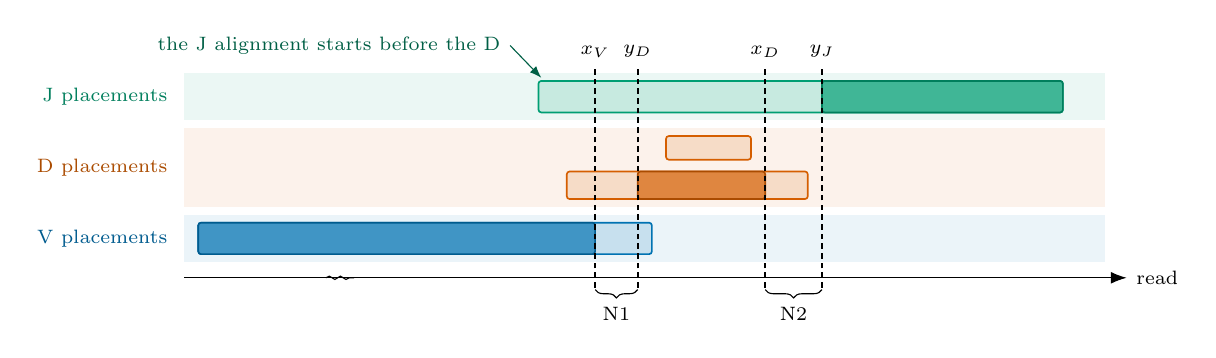
\begin{tikzpicture}[x=0.9mm,y=5mm,font=\small,
    seg/.style={draw=#1,fill=#1!22,line width=0.6pt,rounded corners=1pt},
    kept/.style={draw=#1!80!black,fill=#1!75,line width=0.6pt,rounded corners=1pt},
    cut/.style={draw=black,line width=0.7pt,dash pattern=on 2pt off 1.5pt},
    lab/.style={font=\scriptsize}]
  % lanes (schematic: the junction is drawn wider than to scale)
  \fill[cV!8] (0,0.4) rectangle (130,1.6);
  \fill[cD!8] (0,1.8) rectangle (130,3.8);
  \fill[cJ!8] (0,4.0) rectangle (130,5.2);
  \node[anchor=east,lab,text=cV!80!black] at (-1,1.0) {V placements};
  \node[anchor=east,lab,text=cD!80!black] at (-1,2.8) {D placements};
  \node[anchor=east,lab,text=cJ!80!black] at (-1,4.6) {J placements};
  % read axis
  \draw[-{Latex[length=2mm]}] (0,0) -- (133,0) node[right,lab] {read};
  \draw[decorate,decoration={snake,amplitude=0.6pt,segment length=4pt}] (20,0) -- (24,0);
  % V
  \draw[seg=cV] (2,0.6) rectangle (66,1.4);
  \draw[kept=cV] (2,0.6) rectangle (58,1.4);
  % D (two alleles)
  \draw[seg=cD] (54,2.0) rectangle (88,2.7);
  \draw[kept=cD] (64,2.0) rectangle (82,2.7);
  \draw[seg=cD] (68,3.0) rectangle (80,3.6);
  % J
  \draw[seg=cJ] (50,4.2) rectangle (124,5.0);
  \draw[kept=cJ] (90,4.2) rectangle (124,5.0);
  % cuts
  \foreach \x/\l in {58/x_V,64/y_D,82/x_D,90/y_J} {
    \draw[cut] (\x,-0.25) -- (\x,5.35);
    \node[lab,above] at (\x,5.35) {$\l$};
  }
  % N/P regions
  \draw[decorate,decoration={brace,mirror,amplitude=3pt}] (58,-0.3) -- (64,-0.3)
     node[midway,below=3pt,lab] {N1};
  \draw[decorate,decoration={brace,mirror,amplitude=3pt}] (82,-0.3) -- (90,-0.3)
     node[midway,below=3pt,lab] {N2};
  % annotation of J reaching back over the D
  \node[anchor=east,lab,text=cJ!60!black] (jnote) at (46,5.9) {the J alignment starts before the D};
  \draw[-{Latex[length=1.5mm]},cJ!60!black] (jnote.east) -- (50.4,5.08);
\end{tikzpicture}
\caption{Placements and cuts (schematic; the junction is drawn wider than to scale). Pale bars are candidate local alignments
(placements) of V, D and J alleles to one read; saturated bars are the parts a
path keeps. Between consecutive segments the earlier one exits at $x$, the
later one enters at $y\ge x$, and the bases between are N/P. Overlaps can be
split anywhere or left to N/P. Because nodes are ordered by segment kind, not
by read start, the path V$\to$D$\to$J is available even though the J
alignment reaches back over the D. The placement graph maximises the
objective of \cref{eq:objective} over all such paths, alleles and cut pairs.}
\label{fig:dag}
\end{figure}

\subsection{Objective}
\label{sec:objective}

The score of a path is
\begin{equation}
\begin{aligned}
  \operatorname{score}(\pi) \;=\;& \sum_{\text{segments}} S_{\text{clip}}(\text{segment})
     \;-\; P_V\,\#V \;-\; P_D\,\#D \;-\; P_J\,\#J \\
  &-\; c_{\text{open}}(\text{first}) \;-\; c_{\text{open}}(\text{last})
   \;+\; \sum_{D}\bigl(b\,|D| - \tau_5\,t_5 - \tau_3\,t_3 + \kappa\bigr),
\end{aligned}
\label{eq:objective}
\end{equation}
where $S_{\text{clip}}$ is the score of the kept columns. The other terms are
log prior odds: $P_V$, $P_D$ and $P_J$ in score units, $c_{\text{open}}$ and
the D terms in nats, read at the call's scale (the fixed scale of
\cref{sec:perread} converts $c_{\text{open}}$ to score units and has no D
trim or N/P terms). Each has a stated derivation; the constants it leaves
free (the open-flank allowance, the trim and N/P means and the credit
$\kappa$) were set on simulated reads (\cref{sec:discussion}).

\paragraph{Segment presence.} A D hypothesis is one of $N$ D genes placed at
one of $L$ junction positions, so its prior is spread over $NL$ alternatives.
A maximum a posteriori decision includes the best D when
$\lambda S_D > \ln(NL) - \ln\pi_D$, with $\pi_D$ the prior odds of a D against
none, which gives
\begin{equation}
  \pD \;=\; \frac{\ln(NL) - \ln \pi_D}{\lambda}.
  \label{eq:pd}
\end{equation}
Genes are counted after identical sequences are merged. For the human IGH set
of \cref{sec:evaluation} ($N=30$, $L=25$, even odds) $\pD=10.45$: an exact
5-mer (score 10) loses and an exact 6-mer (12) wins. For TRB ($N=2$)
$\pD=6.17$. V and J pay the same kind of cost over their own genes
($P^{*}_J=7.91$ for its 6 IGHJ genes, $P^{*}_V=12.54$ for its 113 IGHV genes).
Without $P_J$ and
$P_V$, any positive clip completes or starts a path for free, so a read that
stops before its J or starts after its V receives a J or V from a few chance
bases. The cost is kept unrounded; on the integer fixed scale charging
$\lfloor \pD\rfloor$ decides $S>\pD$ exactly. A database of several loci
gives each locus its own costs. An alternative derivation counts the
hypotheses a local D search actually tries, every allele offset and read
position, through the Karlin--Altschul expectation $K w n_D e^{-\lambda S}$
($w$ read positions, $n_D$ allele offsets). It is available as an option
(\code{-{}-d-presence-rate}) but needs a D-presence rate that does not follow
from the search: at the simulator's own rate (0.94) $\pD$ falls below 10 and
exact 5-mers win.

\paragraph{D trims and N/P lengths.} A D clip that keeps germline
$[r_{\text{lo}},r_{\text{hi}})$ of an allele of length $L_a$ trims
$t_5=r_{\text{lo}}$ bases at its 5$'$ end and $t_3=L_a-r_{\text{hi}}$ at its
3$'$ end. Under geometric trims of means 5 and 7 each trimmed base costs
$\tau=\ln((\bar t+1)/\bar t)$, i.e.\ $\tau_5=\ln(6/5)=0.18$ and
$\tau_3=\ln(8/7)=0.13$ nats. Under geometric N/P lengths of mean 8 a junction
pays $\ln(9/8)$ per N/P base, so every read base a D keeps is one N/P base
fewer and earns $b=\ln(9/8)=0.12$ nats. The D cost is credited with
$\kappa=5\tau_5+7\tau_3=1.85$ nats, the trim cost of a D with the prior's mean
trims. The trims then re-rank Ds while a typical D is called as before, and a
short exact match deep inside a long allele, which used to be worth as much
as an untrimmed short allele, pays for the germline it leaves out. Every term
depends on a single cut, through its germline or read position, so a clip
remains worth $\operatorname{exit}(x)-\operatorname{entry}(y)$ and the exact
recursion of \cref{sec:dag} is unchanged.

\paragraph{Open flank.} A path whose last segment is a D asserts a junction
whose J the read does not show in the $x$ bases after the D; one whose first
segment is a D, a V missed in the $x$ bases before it. That D pays the
log-likelihood ratio of those bases under ``no junction, or a junction whose
J (V) was missed'' against ``a junction whose J (V) was missed'':
\begin{equation}
\begin{gathered}
  c(x) = \ln\!\Bigl(1 + \rho\,\frac{1-\varepsilon_{\text{eff}}(x)}{\varepsilon_{\text{eff}}(x)}\Bigr),
  \qquad \varepsilon_{\text{eff}}(x)=\varepsilon\bigl(\min(x-N_{\text{open}},\,64)\bigr),\\
  \varepsilon(\ell) = \max\Bigl(\varepsilon_{\min},\ \min_{1\le\ell'\leq \ell}
     \Pr\bigl[X_{\ell'} \geq k(\ell')\bigr]\Bigr),
  \qquad X_\ell \sim \operatorname{BetaBinomial}(\ell,\,\alpha,\,\beta),
\end{gathered}
\label{eq:openflank}
\end{equation}
where $k(\ell)$ is the number of mismatches among $\ell$ visible bases that
keeps them below the smallest score the missing segment's stage would accept
($\varepsilon=1$ for $\ell\le0$ and while no $\ell$ bases can reach that
score), and $\operatorname{Beta}(\alpha,\beta)$ is the read's mismatch rate
from its anchored V and J columns ($\alpha=k_a+\tfrac12$,
$\beta=n_a-k_a+\tfrac12$ for $k_a$ mismatches among $n_a$ columns).
$\varepsilon(\ell)$ is thus the probability that a segment present in the
read would have stayed below the detection threshold, and the cost is
constant beyond 64 visible bases. The free allowance $N_{\text{open}}=24$ is
the largest 99.9th percentile (22--24 across simulated sets) of the distance
from a called D to the true J start, or from the V end to the D;
$\rho=\tfrac12$ (even odds) and $\varepsilon_{\min}=10^{-3}$ (the anchor
E-value gate) bound the cost to $[0,\,6.2]$ nats. At high divergence a
missing segment could well have been missed and the cost falls accordingly:
with 13 mismatches among 45 anchored columns (about 30\,\% SHM), 64 visible
bases cost 0.99 nats for a missing J and 0.71 for a missing V, against 6.2 on
a clean read. A real D lies within its N/P region of the read end, a chance D
anywhere in the search window, so the cost removes far chance Ds while
keeping real Ds of reads that stop at their D or start in CDR3
(\cref{sec:truncated}).

\paragraph{Order of the decision.} The adjudicator returns the path that
maximises, lexicographically, (1) its value, by default the read's own
log-odds (\cref{sec:perread}); (2) fewer D segments, so a path with a D must
strictly beat the best path without one; and (3) germline \emph{support}, the
sum of its placements' unclipped scores. Key (3) separates paths that explain
the read equally well, typically two alleles of different 3$'$ length at a
junction base that can belong to either side; the allele with more support
admits more cuts with the same score and hence has the larger likelihood
summed over cuts. Co-optimal alleles, equal in clipped score and in matches
and mismatches on the called interval, are all reported. J names are
positional: a tied J allele is named only when it explains the called read
bases at the first allele's own germline coordinates (the same germline
interval), so IGHJ4*02 and IGHJ5*02 trimmed to their
shared 3$'$ part, which tie from different germline offsets, are not both
named; the other remains a tied alternative counted by the posterior.

\subsection{Significance}
\label{sec:significance}

Each V and J hit receives a Karlin--Altschul E-value~\cite{karlin1990}
$E=K w n e^{-\lambda S}$ against its database, with $w$ the length of the
searched read window and $n$ the database length, using exact ungapped

$\lambda$ and $K$ for the scoring in use. A hit is kept only at $E\le 1$, and a
read is \emph{called} only when its path contains an \emph{anchor}: a V or J
hit at $E\le 10^{-3}$ whose clip on that path still reaches the anchor score.
Random sequence therefore receives no call (\cref{sec:specificity}). A J
downstream of a significant V needs only $E\le 1$, since given the V a J is
expected there.

% ===========================================================================
\section{Exact adjudication}
\label{sec:dag}

\subsection{Clipping and separability}

\begin{lemma}[clipping never helps]
\label{lem:clip}
Let $A$ be an optimal local alignment and $A[a..b]$ a contiguous
sub-alignment that begins and ends in match columns. Then
$S(A[a..b])\le S(A)$.
\end{lemma}
\begin{proof}
Every prefix and suffix of an optimal local alignment has non-negative
score, or removing it would give a higher-scoring local alignment. Hence
$S(A[a..b]) = S(A) - S(\text{prefix}) - S(\text{suffix}) \le S(A)$.
\end{proof}

A placement is flattened into columns with prefix scores $P[k]$ and two
tables mapping each read offset to the first match column at or after it and
the last match column before it. A clip to $[lo,hi)$ is then two lookups and
one subtraction, $S=P[\operatorname{exit}(hi)]-P[\operatorname{entry}(lo)]$,
and it is exact because a clip starts and ends on match columns and so never
splits a gap run. The clipped score has one term per cut,
\emph{separability}, and the support key does not depend on the cuts.

\subsection{The recursion}

Placements are the nodes of a lattice, sorted by segment kind (V, D, J) and
then by read start. Every transition between kinds goes forward in this
order wherever the two alignments start, and the cuts alone decide whether
it is feasible ($x\le y$). The paths through a node with a given D count and
first segment kind form a \emph{slot}, which holds one value per canonical
entry cut $y$ of the node: the best key of a path prefix entering there. A
path's first segment keeps its start and its last segment its end, since V
and J are extended outward on purpose; a path can therefore start at a node
only at the node's own start, in the slot whose first kind is the node's.
With a linear N/P score $\iota(y-x)$ ($\iota=0$ by default) the recursion is
\begin{align}
  X(b,x) &= \operatorname{exit}_b(x) - P_{k(b)} + \max_{y\le x-m_b}\bigl[F(b,y)-\operatorname{entry}_b(y)\bigr], \label{eq:rec-exit}\\
  F(e,y') &= \max_b \max_{x\le y'} \bigl[X(b,x) + \iota\,(y'-x)\bigr]
     \quad\bigl(-c_{\text{open}}(e)\text{ at }y'=\operatorname{start}(e)\text{ for a path starting at }e\bigr), \label{eq:rec-entry}\\
  \text{best} &= \max_b\; X\bigl(b,\operatorname{end}(b)\bigr) + \operatorname{end}(g,b) - c_{\text{open}}(b), \label{eq:rec-best}
\end{align}
over every exit $x$ of the predecessor $b$ and every entry $y'\ge x$ of the
successor $e$, where $P_{k(b)}$ is the presence cost of $b$'s kind, $m_b$
its minimum number of retained bases, and $\operatorname{end}(g,b)$ the
whole-path terms of $b$'s slot $g$ (such as an optional V--J pair bonus, 0 by
default). Because each term depends on one cut:
\begin{enumerate}
  \item the best entry for an exit, $\max_{y\le x-m_b}[F(b,y)-\operatorname{entry}_b(y)]$,
    is a running maximum along the node;
  \item the best exit for an entry, $\max_{x\le y'}[X(b,x)-\iota x]$, is a
    second running maximum along $b$, built once per slot of $b$ and per
    successor kind, not per edge;
  \item every entry $y'\ge\operatorname{end}(b)$ sees the same best exit of
    $b$, so the edge $b\to e$ adds it once at $e$'s first entry at or after
    $\operatorname{end}(b)$, and a prefix maximum over $e$'s entries carries
    it to the rest.
\end{enumerate}
An edge therefore costs $O(\text{overlap}+1)$ and a read
$O\bigl(\sum_{\text{slots}}\text{len}+\sum_{\text{edges}}(\text{overlap}+1)\bigr)$,
plus one scan of each node's predecessor slots; \cref{alg:dag} gives the
recursion as pseudocode.
With the open-flank cost on, one transition is barred when the lattice opens
its slots: a V or J none of whose clips pays its presence cost may not
precede or follow a D, since such a placement is no evidence of the
junction's V or J (a junk J of a base or two would otherwise close a D's
flank for less than the cost).
The open-flank cost is a constant of the node and the read added once where a
path starts and once where it ends, and the D priors are added to a D node's
entry and exit prefix values once, when the node is laid out; neither breaks
separability. The recursion is a semi-Markov Viterbi~\cite{viterbi1967,yu2010hsmm}:
segments of variable length scored as wholes, with the cut positions as the
hidden boundaries.

\begin{theorem}
\label{thm:dag}
The recursion of \cref{eq:rec-exit,eq:rec-entry,eq:rec-best} returns the
optimum of \cref{eq:objective}, with the tie order of \cref{sec:objective},
over all grammatical paths (with the transition rule above when the
open-flank cost is on), all placements and all pairs of canonical cuts.
\end{theorem}
\begin{proof}[Proof sketch]
Every grammatical predecessor of a node precedes it in the order by kind, so
by induction over that order $F(e,y)$ is the best value of a path prefix
that enters $e$ at $y$, and $X(b,x)$ that of a prefix that leaves $b$ at $x$.
A path's value is a sum of terms each of which depends on a single cut, so
the maximum over the pair $(x,y)$ of an edge factorises into the two running
maxima above, and the maximum over the entries beyond $b$'s end into one
shifted prefix maximum. Ties are resolved by comparing the lexicographic key
(value, fewer D, support), each of whose parts is separable in the same way.
\end{proof}

\begin{algorithm}[t]
\caption{Exact adjudication of one read. The posterior pass runs the same
loop in the sum-product semiring, with prefix sums in place of running
maxima.}
\label{alg:dag}
\small
\begin{algorithmic}[1]
\Require placements of the read sorted by kind (V, D, J), then read start;
  for each placement $b$ the prefix values $\operatorname{entry}_b(y)$ and
  $\operatorname{exit}_b(x)$ at its canonical cuts, D priors included
\For{each node $e$ in order, and each slot of $e$ (D count, first kind)}
  \State $F(e,y)\gets-\infty$ for every entry $y$
  \If{this is $e$'s start slot and $e$ may start a path}
    \State $F(e,\operatorname{start}(e))\gets -c_{\text{open}}(e)$
  \EndIf
  \For{each predecessor $b$ whose slot and kind may precede $e$}
    \State $F(e,y)\gets\max\bigl(F(e,y),\,M_b(y)+\iota y\bigr)$ for every entry $y<\operatorname{end}(b)$
    \State offer $M_b(\operatorname{end}(b))+\iota y_0$ at the first entry $y_0\ge\operatorname{end}(b)$
  \EndFor
  \State carry the offers to later entries by a prefix maximum, $+\iota$ per base
  \State $G(x)\gets\max_{y\le x-m_e}\bigl[F(e,y)-\operatorname{entry}_e(y)\bigr]$ \Comment{running maximum along $e$}
  \State $X(e,x)\gets\operatorname{exit}_e(x)-P_{k(e)}+G(x)$ for every exit $x$
  \State $M_e(x)\gets\max_{x'\le x}\bigl[X(e,x')-\iota x'\bigr]$, once per kind that may follow $e$
\EndFor
\State \Return $\max_b X(b,\operatorname{end}(b))+\operatorname{end}(g,b)-c_{\text{open}}(b)$ and its trace-back
\end{algorithmic}
\end{algorithm}

The search runs over every canonical entry of the successor, not only those
inside the overlap. Restricting entries to the overlap appears justified by
\cref{lem:clip}, but the lemma bounds prefixes that start at the alignment's
own start, whereas the bases between $b$'s end and a later entry are a
middle stretch of $e$'s alignment and can score below zero: two mismatches
right after the V's end, as a mutated read has, are better left to N/P.
Likewise, ordering nodes by read start alone excludes a D before a J whose
alignment starts earlier. Both restrictions were found by adversarial review
of earlier versions; \swig's test suite now checks \cref{thm:dag} against a
memoised exhaustive enumeration of every grammatical path and canonical cut
pair, on synthetic reads, on the pipeline's own placements for hypermutated
reads, under a two-D grammar (VDDJ optima occur), with the per-read model at
five divergences, with the open-flank cost and with the D priors, and on
constructed reads that each restricted search gets wrong.

\subsection{Calls at the read's own divergence}
\label{sec:perread}

The scores $(2,-3)$ are log-odds only at $11.2\,\%$ divergence. A fixed scale
makes unmutated reads under-confident, since a single nucleotide difference
between two alleles is worth $\ln(3(1-p)/p)=8.0$ nats at $p=0.1\,\%$ rather
than $\lambda\cdot 5=3.2$, and heavily mutated reads over-confident. \swig{}
therefore estimates the read's divergence $\phat$ before adjudication from
the columns no path contests---the best V's match columns before every D and
J placement and the best J's after every V and D placement, N columns
excluded, or all columns of the two placements when fewer than 50
remain---as the Jeffreys predictive rate $(k+\tfrac12)/(n+1)$ for $k$
mismatches among $n$ columns~\cite{jeffreys1946}, clamped to
$[10^{-4},\,0.5]$. Apart from that fallback the junction bases are not among
these columns, so they are not used twice. A substitution column of score
$s\neq 0$ is then worth
$\lambda_r s+\mu_r$ nats, with $(\lambda_r,\mu_r)$ chosen so that a match is
worth $\ln 4(1-\phat)$ and a mismatch $\ln(4\phat/3)$; at $\phat=\delta$,
$\lambda_r=\lambda$ and $\mu_r=0$. Gaps stay at the prior $\lambda$, since
$\phat$ measures substitutions.

Every term is an integer in units of $1/F$ nats, $F=2^{16}$: a column is
$s\,u_r+v_r$ with $u_r=\operatorname{round}(F\lambda_r)$ and
$v_r=\operatorname{round}(F\mu_r)$, so the maximum and every tie are exact,
and the recursion and \cref{thm:dag} carry over unchanged. At
$\phat=\delta$ every column is the fixed score times
$u_0=\operatorname{round}(F\lambda)$, so with integer presence costs and the
D priors off the fixed scale (\code{-{}-calls fixed}, which has no D trim or
N/P terms) is an exact special case. The D cost is read as $\pD/m$ matched D
columns, with $m$ the D match score,
\begin{equation}
  c_D(\phat) = \Bigl\lfloor \pD\,\frac{m u_D+v_D+\operatorname{round}(F b)}{m}\Bigr\rfloor - \operatorname{round}(F\kappa),
\end{equation}
rather than as a constant number of nats. The cost is a threshold against
chance D hits in random N/P sequence, whose null distribution does not depend
on $\phat$ and is dominated by exact runs. Read in matched columns it keeps
the fixed scale's admitted classes of exact runs at every divergence for a D
with the prior's mean trims (runs of 5 lose, runs of 6 win when their trims
cost $\kappa$); the trim terms move runs that are trimmed less or more than
that across the threshold. A cost constant in nats would instead admit
exact 5-mers on unmutated reads whatever their trims.

\subsection{Posterior probabilities}
\label{sec:posterior}

The objective is a log-likelihood ratio, so it also defines a distribution
over every grammatical path and every pair of canonical cuts,
\begin{equation}
  P(\pi,\text{cuts}\mid q) = \frac{\exp\bigl(\operatorname{nats}(\pi,\text{cuts})\bigr)}{Z}.
\end{equation}
Forward--backward~\cite{rabiner1989,durbin1998} over the same lattice---the
sum-product twin of \cref{eq:rec-exit,eq:rec-entry,eq:rec-best}, with prefix
and suffix sums where the Viterbi pass has running maxima---gives the marginal
of every placement and of every D count in the same $O(\text{overlap}+1)$ per
edge. Under the default call both passes read the same integer model, so the
Viterbi path is a mode of the reported distribution. A segment's reported
posterior is the mass of every placement of its kind that is tied with the
call on the called interval or explains most of the called bases with
germline the primary allele contains; the event is ``the reported names
include the read's allele, up to germline equivalence'', which is exactly
what the evaluation scores (\cref{sec:evaluation}). The read's D-presence
probability is $1-P(\text{no D})$.

The arithmetic is linear with one log-scale per slot, as in scaled HMM
recursions. Cut weights are running products along the alignment, so no
transcendental function is evaluated per cut; entry and exit weights are
centred separately; the N/P factor is accumulated as a relative recursion
whose factors are $\le 1$; and the cost of a gap between non-overlapping
neighbours joins the slot's log-scale rather than multiplying it. A read
whose evidence would leave the range of double precision (a placement
spanning more than 1,200 nats on one side, or an overlap gaining more than
600) receives no posterior rather than a wrong one. Tests compare the
marginals with exhaustive summation under VJ, VDJ and VDDJ grammars, with
N/P costs, N columns, insertions, long costly gaps, the open-flank cost and
the D priors.

An optional decoder (off by default) takes a call with exactly one D and
finds the allele of largest posterior marginal,
$a^{*}=\argmax_a\sum_{p\ni a}P(p)$ over D placements $p$; the marginal is
not conditioned on the call's topology. When $a^{*}$ beats the call's
allele, the path is re-traced with the call's first and last kind and D
count on the lattice masked to the V and J placements and $a^{*}$'s D
placements, and kept when it stays anchored and its reported D posterior is
no lower.


% ===========================================================================
\section{Plausibility constraints}
\label{sec:guards}

On full-length simulated reads the optimum of \cref{eq:objective} almost
always pairs a V and a J that could form one rearrangement, but on
truncated, chimeric and cross-locus reads it need not. \swig{} applies, as
constraints outside the objective and on by default, the plausibility checks
of SwiftIG, an earlier C++ aligner (unpublished) whose method note \swig{}
began as a Rust implementation of: minimum hit lengths of 24 (V) and 10 (J)
local alignment columns; a V--J pairing rule (the V and J face their
junction, hold a long split, or align both conserved codons in order), to
which \swig{} adds that a V shorter than 80 columns pairs only with a J that
is significant on its own; and a span of at most 225 bases between the V's
exit and the J's entry. SwiftIG called a D only between a V and a J that
pair. \swig{} also admits a D beside a V or a J alone, but only when it pays
the open-flank cost and lies within 60 bases of the segment the read shows.
The call is the unconstrained optimum when it satisfies the constraints;
otherwise the lattice is re-adjudicated over subsets of placements (the V
placements alone, the J placements alone, and each J with the V placements
it pairs with, with and without the Ds; under the open-flank cost also V and
D placements within reach of each other, and D and J placements), and the
call is the best admissible subset optimum. Within each subset the key is the
exhaustive optimum, but a subset whose optimum breaks a constraint
contributes nothing, so the guarded call is \emph{defined} rather than exact.
On the test suite's 435 checked calls, no admissible path over any choice of
at most one V, D and J among a read's best 4, 8 and 4 placements beat the
call under the per-read model (one did under the fixed scale). Junctions are
reported only from conserved anchors

(Cys104, Trp/Phe118) that the called alignments actually align, with a
bounded recovery of a Cys104 lying just past a clipped V end.

% ===========================================================================
\section{Search}
\label{sec:search}

Each stage narrows the hypotheses the lattice sees. \Cref{tab:search} states
what each step can lose: \emph{exact}; \emph{lossless}, which provably drops
nothing the model could choose; \emph{bounded}, which drops only what lies
outside a stated geometric bound; \emph{defined}, a stated selection rule
whose output is the definition of the result rather than an approximation
of an optimum; \emph{approximate}, a known gap to the model's optimum; and
\emph{heuristic}, which is measured, not proven. \Cref{fig:pipeline} shows
the flow.

\begin{figure}[t]
\centering
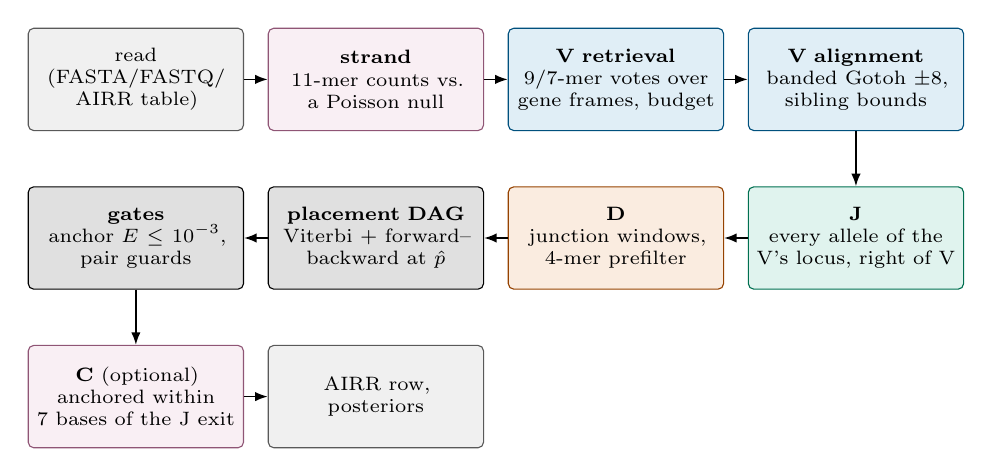
\begin{tikzpicture}[font=\scriptsize,node distance=3mm and 3mm,
  box/.style={draw,rounded corners=2pt,align=center,minimum height=13mm,text width=25mm,fill=#1!12,draw=#1!70!black},
  arr/.style={-{Latex[length=1.6mm]},line width=0.6pt}]
  \node[box=gray] (read) {read\\(FASTA/FASTQ/\\AIRR table)};
  \node[box=cOff,right=of read] (strand) {\textbf{strand}\\11-mer counts vs.\\a Poisson null};
  \node[box=cV,right=of strand] (vret) {\textbf{V retrieval}\\9/7-mer votes over\\gene frames, budget};
  \node[box=cV,right=of vret] (valn) {\textbf{V alignment}\\banded Gotoh $\pm 8$,\\sibling bounds};
  \node[box=cJ,below=7mm of valn] (j) {\textbf{J}\\every allele of the\\V's locus, right of V};
  \node[box=cD,left=of j] (d) {\textbf{D}\\junction windows,\\4-mer prefilter};
  \node[box=black,left=of d] (dag) {\textbf{placement DAG}\\Viterbi + forward--\\backward at $\hat p$};
  \node[box=black,left=of dag] (guard) {\textbf{gates}\\anchor $E\le10^{-3}$,\\pair guards};
  \node[box=cC,below=7mm of guard] (c) {\textbf{C} (optional)\\anchored within\\7 bases of the J exit};
  \node[box=gray,right=of c] (out) {AIRR row,\\posteriors};
  \draw[arr] (read) -- (strand);
  \draw[arr] (strand) -- (vret);
  \draw[arr] (vret) -- (valn);
  \draw[arr] (valn) -- (j);
  \draw[arr] (j) -- (d);
  \draw[arr] (d) -- (dag);
  \draw[arr] (dag) -- (guard);
  \draw[arr] (guard) -- (c);
  \draw[arr] (c) -- (out);
\end{tikzpicture}
\caption{Pipeline of one read. The V, J, D and C alignment stages run over
chunks of 64 reads on the inter-sequence SIMD kernel (16 or 32 lanes); strand,
windows, admission, adjudication and the gates are decided per read.
\Cref{tab:search} gives the guarantee of each step.}
\label{fig:pipeline}
\end{figure}

\begin{table}[t]
\centering
\caption{Search steps and what each can lose.}
\label{tab:search}
\small
\begin{tabularx}{\linewidth}{@{}l l X@{}}
\toprule
Step & Guarantee & Rule and justification \\
\midrule
Strand & heuristic & Count read positions whose 11-mer occurs in the V/J germline on each strand; trusted when the winner exceeds its Poisson null $\lambda_0+3\sqrt{\lambda_0}$ ($\lambda_0$: the read's $k$-mer count times the germline's 11-mer density), otherwise compare V seed votes on both strands. \\
V retrieval & heuristic & Seed votes per gene frame (9-mers weight 4; 7-mers weight 1 while the leader holds fewer than 25 nine-mer seeds). Keep 3 genes, and up to 16 while their votes are within $z\sqrt{2\cdot 4\cdot L}$ of the leader's $L$, $z=2$: about two standard deviations of the difference of two seed counts, so the margin is proportionally wider for weakly supported, mutated reads. Every allele of a kept gene is a candidate. \\
V band & bounded & The seed cluster's diagonal range $\pm 8$, spanning both clusters around a seeded indel; holds unless an indel longer than 8 escapes the seeds. \\
V, J scoring & lossless & One representative $R$ per gene frame is aligned; a sibling $A$ satisfies $\underline{L}\le S^{*}(A)\le S^{*}(R)+\Delta(R,A)$ and is skipped when the upper bound is below the third-largest lower bound. The ranking from the third score up equals full scoring. \\
V/J keep & defined & Top 3 by extended and top 3 by local score with $E\le1$, plus ties. \\
J & bounded & Every J allele of the anchoring V's locus, unbanded, from 12 bases before the earliest V end to at most 225 bases plus the longest J past the last anchoring V's end; the whole read when no V is an anchor. \\
D windows & bounded & $[\text{V end}-12,\ \text{J start}+12)$ from the best anchoring V and the best J placement, plus the conserved-anchor window $[\text{Cys104}+3,\ \text{Trp/Phe118})$; an open side reaches 60 bases. \\
D prefilter & lossless & An allele is aligned only if it shares an $\ell$-mer with the window, $\ell$ derived from the admission gate (exact run $\ge 4$). \\
D alignment & approximate & One optimal local alignment per allele and window, the best 32 admissible ones (plus ties) per window; its clip at the chosen cuts need not be the best clip of that allele. \\
Adjudication & exact & \Cref{thm:dag}. \\
Guards & defined & Best admissible subset optimum (\cref{sec:guards}). \\
C & exact within 7 bases & Anchored DP at the J exit (\cref{sec:constant}). \\
\bottomrule
\end{tabularx}
\end{table}

\paragraph{Gene frames and the index.} The alleles of a gene share almost
all seeds. An allele joins its gene's coordinate frame when at least 30\,\%
of its seeds occur in the gene's longest allele and every one of those
shared seeds agrees on one offset; SNP and truncated alleles join, an allele with an
internal indel gets its own frame. The $k$-mer index is built over frames in
compressed-sparse-row form, with 2-bit packed keys used directly as array
indices, so a seed shared by twenty alleles is one posting and one vote and
retrieval work scales with genes rather than alleles. Votes are packed into
64-bit integers and radix-sorted in linear time; one scan then yields the
best diagonal cluster per frame. Seeds with more than 256 postings are
skipped, and a seed repeated within a frame does not vote, so repeats cannot
collect quadratic votes. We measured closed and open syncmers and
minimisers~\cite{edgar2021syncmers,shaw2022syncmers} as seed samplers
(minimisers only under an earlier fixed gene margin). Under the noise-based
margin every $k$-mer beat closed syncmers by 1.1 points of mean V gene
accuracy (4.4 at 30\,\% SHM) for 0.4\,\% more instructions, and beat open
syncmers too, so it is the default.

\paragraph{Sibling bounds.} For a sibling $A$ aligned in the same frame
diagonals as its representative $R$, $\Delta(R,A)$ sums the best profile gain
at each frame position both alleles cover and the best substitution score
where only $A$ does, so $S^{*}(A)\le S^{*}(R)+\Delta(R,A)$. The lower bound
$\underline{L}$ rescores a traced representative path clipped to $A$'s span
with $A$'s profile, in time proportional to the positions where the two
differ. A sibling whose bounds meet needs no alignment, and one whose lower
bound already reaches the cut-off is aligned outright with its traceback
reused. Because the cut-off is a lower bound on the true third score, the
kept ranking is that of aligning every allele.

\paragraph{D search.} The junction windows reclaim 12 bases into V and J,
and the conserved-anchor window depends on where the J's Trp/Phe118 lands,
not on how far its alignment reaches left; with the lattice's ordering by
kind, the read's own J cannot remove its D from consideration. A chance J
placement between the V and the D of a read that stops at its D can, since
the window ends 12 bases after the best J placement, used or not. Each D
allele sharing an $\ell$-mer with a window is aligned there, unbanded, and
its optimal local alignment competes for the 32 places (plus ties) that the
window's admissible D hits have in the lattice. D admission requires an
exact run of at least 4 bases; 3, 5 and 6 were measured and are worse.

\subsection{Constant region}
\label{sec:constant}

With a C database the constant region is assigned after adjudication, from
finished calls only, so V, D and J calls are unchanged by construction. J and
C are joined by an RNA splice at fixed phase, so C's germline base 0 lies at
the called J's exit $x$, up to reference conventions and indels near the J's
3$'$ end; hypothesis $H(a,o)$ places base 0 of allele $a$ at $x+o$,
$|o|\le 7$. An alignment anchored at $C[0]$ on one of these 15 diagonals is
computed exactly by any local aligner run on $[N]+C$ whose first column
scores a bonus larger than any alignment avoiding it, so the SIMD kernel
serves unchanged. Alleles whose sequences agree on the reachable prefix form
reach classes and are aligned once (the IMGT human IGHC set used here has 105
distinct alleles but only 13 distinct 32-nt prefixes). C is called when its
anchored E-value $E_C=15\,N_C\,e^{-\lambda S}\le 10^{-3}$, with $N_C$ the
number of C genes of the J's locus, from a Lundberg-type bound for the
walk from each start, on at least 12 aligned columns at 90\,\% identity, and
its posterior is computed at C's own divergence, since C is not
hypermutated.

\subsection{Germline annotation}

Conserved anchors fix every reading frame and junction end: V Cys104 and J
Trp/Phe118. They and the V region boundaries are settled once per database,
in order of trust: header keys, IMGT-gapped numbering when the gaps are
consistent, a joint motif search for Cys23, Trp41 and Cys104, transfer from
the most similar allele by local alignment, and finally database models: a
Jeffreys-smoothed model of the FR3 length given the Trp41--Cys104 spacing,
and of the Cys23 position. Every derived value that may be wrong carries an
\emph{uncertain} flag, so an error without the flag is a silent error. Each
allele's locus is read from its name or inferred from its relatives and,
failing that, from an embedded panel of human and mouse family
representatives; the locus decides which alleles may form one
rearrangement and which gene counts price a segment. V alleles named
without the \code{*} allele separator join the gene of their nearest named
relative ($\ge 0.95$ of the smaller self-score; the rest are grouped among
themselves), so the gene-level retrieval budget does not silently become an
allele cap.


% ===========================================================================
\section{Implementation}
\label{sec:implementation}

\swig{} is a Rust crate (edition 2024, Rust $\ge 1.89$) with no dependencies:
about 38,000 lines of library code with inline unit tests, 5,400 lines of
integration tests and 1,300 of examples and WebAssembly bindings. Every component is a statically
dispatched trait---aligner, retrievers, candidate budget, substitution model,
D window policy, admission, adjudicator, grammar and path model---so swapping
one changes the type and the pipeline monomorphises without trait objects.

\paragraph{Inter-sequence SIMD.} Following Rognes~\cite{rognes2011}, each
16-bit lane runs the scalar Gotoh recurrence for a different read--allele job
rather than striping one alignment~\cite{farrar2007}. The kernel is written
once over a lane abstraction and compiled for AVX-512BW (32 lanes), AVX2,
NEON, WebAssembly~\cite{haas2017wasm} \code{simd128} and portable lanes (16).
By default the fastest of AVX2, NEON and portable lanes is chosen at run time;
AVX-512BW runs only on request (\code{-{}-simd avx512}), since 512-bit
instructions lower the clock of many CPUs. On WebAssembly the backend is
fixed at build time (\code{simd128}, or the scalar kernel without it).
Banded jobs use band-relative coordinates, so lanes whose
bands start on different diagonals walk the same grid~\cite{chao1992band}.
When every lane's profile depends on base identity alone a cell's
substitution is one comparison and one blend; otherwise five profile rows are
selected by mask, exact for any substitution model. The horizontal gap state
uses $D'=\max(t+g_o,\,D+\max(g_o,g_e))$ with $t=\max(0,\text{diag},I)$, which
shortens the loop-carried dependency to one add and one maximum and is exact
for any gap costs. Arithmetic saturates in 16 bits; a job enters a lane only
if its attainable local score is at most 30,000, no step costs less than
$-1{,}000$ and its dimensions fit 16-bit positions, so saturation never clips
a real cell, and other jobs run on the scalar kernel.
Traceback codes are bit-identical to the scalar kernel's, so one traceback
walk serves both.

\paragraph{Batching and determinism.} Each stage runs over a chunk of 64
reads, giving one score batch and a few traceback waves per stage, while
every decision stays per read; a read's result does not depend on its chunk,
which is tested. Threads self-schedule chunks from an atomic counter with
one workspace each, so there is no allocation in the DP after warm-up, and
results return in input order. The scalar kernel equals a textbook Gotoh,
every SIMD backend equals the scalar kernel in scores, end cells and
tracebacks, the batched pipeline equals the per-read scalar pipeline, and
output is byte-identical across backends and between x86-64 and AArch64.

\paragraph{Input, output and interfaces.} Reads are FASTA, FASTQ or an AIRR
Rearrangement table, streamed in batches of 16,384; identical sequences are
assigned once per batch, and across batches through a cache of the 4,096
most recently assigned distinct sequences, which changes no output. Output is
the AIRR Rearrangement schema~\cite{vanderheiden2018airr} with the
posteriors, E-values, alternatives and region coordinates. The crate provides
a command line (\code{swig}, with \code{prepare}, \code{simulate} and
\code{evaluate} subcommands) and a Rust library; a companion workspace crate
(\code{swig\_wasm}) builds a WebAssembly module with a C ABI. All three share
one run implementation.

\paragraph{Tests.} The suite of 350 tests, all passing on the version
described (one long-running accuracy test of 20,000 reads per preset runs on
demand), includes the exhaustive oracles for \cref{thm:dag} and the
posterior marginals, kernel equivalence on random batches for every backend
the host runs (AVX-512BW, AVX2 and portable lanes on x86-64; NEON and
\code{simd128} on AArch64 and WebAssembly builds), the guards on constructed
reads, robustness on
degenerate input (empty, all-N, IUPAC, low-complexity, 20\,kb and chimeric
reads, and every prefix and suffix of a read), and accuracy floors on
simulated reads. It runs on release code with debug assertions and overflow
checks enabled.

% ===========================================================================
\section{Evaluation}
\label{sec:evaluation}

All reads in this paper are simulated, so that every call can be scored
against a known answer; none of the results is external biological
validation (\cref{sec:discussion}). Two independent simulators are used. The
numbers in \cref{sec:results} were produced with \swig{} 0.39.7 for this
paper, except the MiXCR results and the D-prior prototype measurements of
\cref{sec:genairr}, which come from an earlier run of the GenAIRR benchmark
on the same reads.

\paragraph{GenAIRR.} GenAIRR 2.3.1~\cite{konstantinovsky2024genairr}
simulates reads with its built-in references (human IGH from
OGRDB~\cite{lees2020ogrdb}: 198 V, 33 D and 7 J alleles; IGK 168 V and 8 J;
IGL 181 V and 10 J; TRB 98 V, 3 D and 16 J), 10,000 reads per set, seed 7,
forward strand. Scenarios are unmutated (\emph{naive}); S5F
mutation~\cite{yaari2013s5f} at 2, 5 and 10\,\%; and \emph{realistic}: S5F at
5\,\% with a 5$'$ primer trim of 0--15 and a 3$'$ trim of 0--5 bases, 0--1
polymerase indels, 0.2\,\% PCR and 0.2\,\% sequencing errors and 0--2 N calls
(for TRB, the same artefacts without SHM). Every tool receives the GenAIRR
reference: \swig{} with each allele's anchor in its header, IgBLAST as
\code{makeblastdb} databases with a J auxiliary file, MiXCR as a repseqio
library. GenAIRR's truth for each segment is a \emph{tie set}: each allele
earns a point for every read base that matches it at the same germline index
as the sampled allele, over the segment's true read region, and every allele
at the maximum is in the set. A call $C$ against truth $T$ scores the Jaccard
index $|T\cap C|/|T\cup C|$ per read and segment (both empty scores 1, one
empty 0), and tables give the mean in \%. One correct allele against a
two-allele tie therefore scores $\tfrac12$, as does a two-allele call against
a one-allele truth.

\paragraph{IgSim.} \swig{} ships a dependency-free Rust port of the
generative model and presets of IgSim.jl~\cite{igsimjl}: uniform allele
choice, exonuclease trims, N additions, random flanks, gated SHM with
single-base indels, and instrument substitutions, with every read base
labelled by its germline origin. The presets are \emph{easy} (no SHM),
\emph{mid} (IgM-like: SHM on 40\,\% of reads at 0.5--7\,\%; 1-nt indels
switched on for 8\,\% of reads at up to 0.2\,\% per base, so about 2\,\% carry
one) and \emph{hard} (IgG-like: SHM on 97\,\% of reads, median about 7\,\%;
indels on 15\,\% at up to 0.4\,\% per base, about 7\,\% carry one); we also run
the \emph{hard} preset with the SHM rate fixed at 30\,\% on every read to
probe the extreme.
The germline is the human IGH set of IMGT/GENE-DB~\cite{giudicelli2005genedb}
release 202632-7 (480 V, 48 D and 15 J alleles, of which \swig{} merges
identical sequences to 457, 41 and 15), given to every tool as plain FASTA:
\swig{} annotates the anchors itself. The simulator draws only V and J alleles
with a trusted anchor, since a junction truth built on a guessed anchor would
rest on the annotation it is meant to test. An allele call is correct when it
is \emph{germline-equivalent} to the truth: the called allele contains the
trimmed, pre-mutation germline that was simulated, so no method could
separate the two from the read. Junctions are correct when they equal the
true Cys104--Trp/Phe118 sequence; junction accuracy is over the reads whose
two anchor codons are templated in the read (9,953, 8,130 and 4,667 of
10,000 on \emph{easy}, \emph{mid} and \emph{hard}; 1,441 of 3,000 at 30\,\%
SHM). Because the trade-off between finding short
D remnants and leaving D-free junctions without a D can be moved at will, D
accuracy is always reported together with the share of D-free reads that are
given a D, and by remnant length.

\paragraph{Comparisons and statistics.} Two callers or settings are compared
on identical reads. For each metric \code{swig evaluate}, which scores any
AIRR Rearrangement table and so serves every tool alike, computes the
accuracy difference with its 95\,\% paired Wald interval and an exact
two-sided McNemar test~\cite{mcnemar1947} on the reads only one of them gets
right; we report the differences and the McNemar $p$-values.
 Posteriors are scored by reliability bins, the expected
calibration error~\cite{naeini2015ece}
$\text{ECE}=\sum_b n_b\,|\bar p_b-\bar e_b|/n$ and the Brier
score~\cite{brier1950}.

\paragraph{Tools and hardware.} IgBLAST 1.22.0 (Bioconda) was run with the
options \code{-organism human}, \code{-ig\_seqtype Ig} (\code{TCR} for TRB)
and \code{-outfmt 19}, with custom V, D and J databases built from the same FASTA.
Its auxiliary file lacked IGHJ5*03 and IGHJ5*04 of the IMGT set; we added
them with the frame and CDR3 end of IGHJ5*01, which \swig{}'s anchors
reproduce. MiXCR 3.0.13, the last release that runs without a licence key,
was run with \code{align} and \code{exportAlignments}, and is reported
counting every hit tied with its top score, the fairer comparison with tools
that list co-optimal alleles. Its figures come from an earlier run of the
same GenAIRR benchmark on identical reads: the simulations are seeded, and
our regenerated IgBLAST and \swig{} scores on them reproduce that run's to
the last reported digit. \swig{} 0.39.7 ran with its default profile.
All timings are wall-clock times of the whole command on a 4-vCPU Intel Xeon
virtual machine at 2.1\,GHz (AVX-512BW) with 15\,GB of memory, on four threads
unless stated.

% ===========================================================================
\section{Results}
\label{sec:results}

\subsection{Accuracy against ambiguity-aware truth}
\label{sec:genairr}

\Cref{tab:genairr} compares the three tools on GenAIRR reads. \swig{} has
the highest V, D and J score on every human IG set. The margin is largest
for IGH D and grows with mutation (\cref{fig:genairr}): from 0.7 points over
IgBLAST on unmutated reads to 6.0 points at 10\,\% SHM, and 2.4 points on
the realistic set. MiXCR's top-tied hits trail on D by 3.9--9.2 points over
the IGH sets; its single top hit, which drops genuine ties, scores lower
still (IGH D 73.5--86.4\,\%, V 94.6--99.6\,\%). On TRB \swig{} has the best D
(99.9 and 99.5\,\% against at most 98.2\,\%) but trails IgBLAST and MiXCR by
0.04--0.11 points on J: on a few reads the J is trimmed 31--40 bases into its
germline, past its Trp/Phe codon, and its 13--22 remaining bases fail the V--J
pairing rule of the plausibility constraints (the J starts more than 30 bases
into its germline, holds fewer than 30 columns and aligns no conserved
codon).

\begin{table}[t]
\centering
\caption{Accuracy against GenAIRR's ambiguity-aware truth (mean Jaccard
score of the reported allele set against the truth's tie set, \%), 10,000
reads per set. MiXCR counts every hit tied with its top score; its figures
come from an earlier run of the benchmark on the same reads. Bold: best of
the row. A dash: the locus has no D.}
\label{tab:genairr}
\footnotesize
\setlength{\tabcolsep}{3.2pt}
\begin{tabular}{@{}l rrr rrr rrr@{}}
\toprule
 & \multicolumn{3}{c}{IgBLAST 1.22} & \multicolumn{3}{c}{MiXCR 3.0.13} & \multicolumn{3}{c}{\swig{} 0.39.7} \\
\cmidrule(lr){2-4}\cmidrule(lr){5-7}\cmidrule(l){8-10}
Set & V & D & J & V & D & J & V & D & J \\
\midrule
IGH, no SHM      & 99.86 & 97.80 & 99.48 & 99.76 & 94.56 & 99.53 & \textbf{99.98} & \textbf{98.47} & \textbf{99.76} \\
IGH, 2\,\% SHM   & 99.80 & 96.55 & 99.36 & 99.65 & 93.34 & 99.37 & \textbf{99.85} & \textbf{97.28} & \textbf{99.70} \\
IGH, 5\,\% SHM   & 99.64 & 93.24 & 99.14 & 99.30 & 90.22 & 98.81 & \textbf{99.67} & \textbf{95.42} & \textbf{99.47} \\
IGH, 10\,\% SHM  & 99.36 & 84.28 & 98.48 & 98.45 & 81.07 & 96.60 & \textbf{99.43} & \textbf{90.24} & \textbf{99.06} \\
IGH, realistic   & 99.53 & 92.56 & 99.05 & 99.01 & 89.55 & 98.73 & \textbf{99.60} & \textbf{94.96} & \textbf{99.44} \\
IGK, 5\,\% SHM   & 99.63 & -- & 98.88 & 99.14 & -- & 98.35 & \textbf{99.74} & -- & \textbf{99.43} \\
IGK, realistic   & 99.48 & -- & 98.11 & 97.99 & -- & 97.09 & \textbf{99.63} & -- & \textbf{99.02} \\
IGL, 5\,\% SHM   & 99.53 & -- & 98.32 & 98.48 & -- & 98.16 & \textbf{99.63} & -- & \textbf{99.10} \\
IGL, realistic   & 99.34 & -- & 98.32 & 97.16 & -- & 96.49 & \textbf{99.51} & -- & \textbf{98.49} \\
TRB, no SHM      & \textbf{99.97} & 98.17 & 99.93 & 99.94 & 94.10 & \textbf{100.00} & \textbf{99.97} & \textbf{99.91} & 99.89 \\
TRB, realistic   & \textbf{99.94} & 97.65 & \textbf{99.92} & 99.80 & 93.66 & \textbf{99.92} & \textbf{99.94} & \textbf{99.50} & 99.87 \\
\bottomrule
\end{tabular}
\end{table}

\begin{figure}[t]
\centering
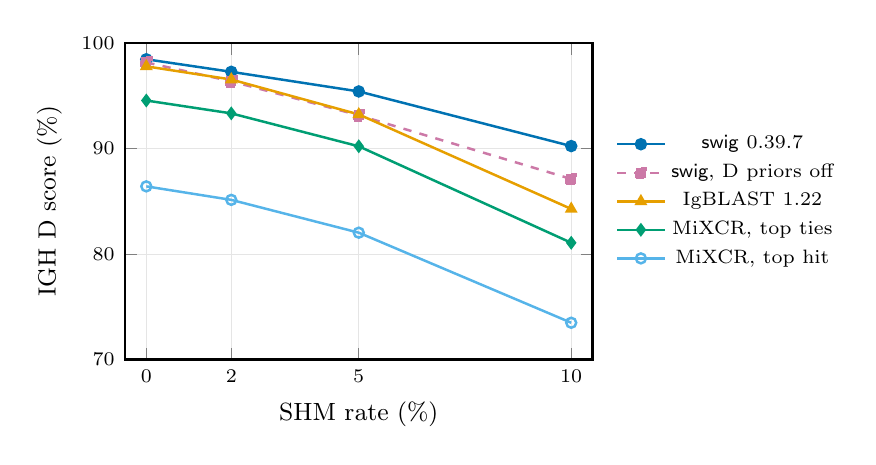
\begin{tikzpicture}
\begin{axis}[width=0.62\linewidth,height=5.6cm,
  xlabel={SHM rate (\%)},ylabel={IGH D score (\%)},
  xtick={0,2,5,10},ymin=70,ymax=100,xmin=-0.5,xmax=10.5,
  legend style={font=\scriptsize,at={(1.03,0.5)},anchor=west,draw=none},
  tick label style={font=\scriptsize},label style={font=\small},
  grid=major,grid style={gray!20},mark size=1.8pt,line width=0.9pt]
\addplot[cSwig,mark=*] coordinates {(0,98.47) (2,97.28) (5,95.42) (10,90.24)};
\addlegendentry{\swig{} 0.39.7}
\addplot[cOff,mark=square*,dashed] coordinates {(0,98.17) (2,96.38) (5,93.16) (10,87.12)};
\addlegendentry{\swig, D priors off}
\addplot[cIgb,mark=triangle*] coordinates {(0,97.80) (2,96.55) (5,93.24) (10,84.28)};
\addlegendentry{IgBLAST 1.22}
\addplot[cMix,mark=diamond*] coordinates {(0,94.56) (2,93.34) (5,90.22) (10,81.07)};
\addlegendentry{MiXCR, top ties}
\addplot[cMixTop,mark=o] coordinates {(0,86.42) (2,85.14) (5,82.03) (10,73.49)};
\addlegendentry{MiXCR, top hit}
\end{axis}
\end{tikzpicture}
\caption{Human IGH D accuracy on GenAIRR reads as SHM increases (mean
Jaccard score against the truth's tie set). ``D priors off'' is \swig{} 0.39.7
with \code{-{}-d-trim off -{}-np-length off}, which reproduces the D calls of
the previous release.}
\label{fig:genairr}
\end{figure}

\paragraph{Where the D gain comes from.} Without its D trim and N/P-length
priors \swig{} 0.39.7 makes the D calls of its previous release, which was
level with IgBLAST at 2 and 5\,\% SHM (\cref{fig:genairr}). An analysis of that
release's errors on a 2,000-read sample of the 5\,\% SHM set found that 95 of
its 103 wrong-gene D calls overlapped the true D: the D had been found, but a
short exact match of
another gene inside a mutated true D (for example \code{CTACAAT} inside
\code{ACTACAATAA}) outscored it by local alignment. A post-processing
prototype that held the placement graph's V end and J start fixed and
re-decided the D under a posterior over allele, offset and both trims showed
that the gain came from the trim and N-length priors and not from a
different decision rule or hypothesis space: with flat priors it matched the
graph's D calls (93.12 against 93.16 at 5\,\% SHM), and restricting each
allele to one offset, as the graph does, cost at most 0.1 point. Moving both
priors into the graph as cut terms (\cref{sec:objective}) recovered most of
the prototype's gain (95.42 against 95.67 at 5\,\% SHM) at 0.6\,\% more
instructions, whereas the prototype as a separate pass would have added
37--47\,\% to the run time.

Because the priors were designed on these reads, we simulated four IGH
scenarios again from a disjoint part of GenAIRR's random stream, sharing no
read with the sets above (\cref{tab:oos}). The picture is unchanged: the
priors add 0.5--3.4 points of D, at least as much as on the design sets, and
\swig{} leads IgBLAST on V, D and J in every scenario, on D by 0.9--6.3
points.

\begin{table}[t]
\centering
\caption{Out-of-sample check: GenAIRR human IGH reads disjoint from those of
\cref{tab:genairr} (10,000 per scenario; mean Jaccard score, \%). ``Priors
off'': \swig{} 0.39.7 with \code{-{}-d-trim off -{}-np-length off}.}
\label{tab:oos}
\footnotesize
\begin{tabular}{@{}l rrr r rrr@{}}
\toprule
 & \multicolumn{3}{c}{\swig{} 0.39.7} & priors off & \multicolumn{3}{c}{IgBLAST 1.22} \\
\cmidrule(lr){2-4}\cmidrule(lr){5-5}\cmidrule(l){6-8}
Scenario & V & D & J & D & V & D & J \\
\midrule
no SHM     & 99.98 & 98.40 & 99.65 & 97.89 & 99.82 & 97.54 & 99.48 \\
5\,\% SHM  & 99.66 & 94.97 & 99.39 & 92.71 & 99.59 & 92.65 & 99.15 \\
10\,\% SHM & 99.46 & 90.20 & 98.97 & 86.82 & 99.44 & 83.94 & 98.47 \\
realistic  & 99.54 & 94.75 & 99.33 & 92.43 & 99.44 & 92.12 & 99.13 \\
\bottomrule
\end{tabular}
\end{table}

\subsection{Germline-equivalent accuracy, D-free junctions and junctions}
\label{sec:igsim}

\Cref{tab:igsim} compares \swig{} and IgBLAST on IgSim reads against the
IMGT human IGH set, read by read. \swig{} calls the V allele more often
correctly on unmutated, IgM-like and IgG-like reads ($p<10^{-6}$ each), the D
allele on unmutated and IgG-like reads ($+2.2$ points on \emph{hard},
$p=10^{-13}$), and the J allele on IgG-like reads, while giving a D to far
fewer D-free junctions (18.4 against 49.4\,\% on \emph{mid}, 15.8 against
30.8\,\% on \emph{hard}). On remnants of 8 or more nucleotides \swig's D is
better on every preset. IgBLAST's 0.5-point higher D accuracy on \emph{mid}
($p=0.017$) comes entirely from remnants of 1--3 nucleotides (74.3 against
36.6\,\%), which no method can identify: almost any allele containing the
remnant is germline-equivalent to it, so a tool that always calls a D is
credited there, and pays for it on D-free junctions.

IgBLAST reports more exact junctions (99.94 against 99.53\,\% on \emph{mid},
98.33 against 96.81\,\% on \emph{hard}). This is the cost of \swig's
plausibility constraints, which report a junction only from conserved
anchors that the called V and J alignments actually align: without them
\swig's junctions are 99.98 and 99.66\,\% exact (\cref{tab:ablation}), above
IgBLAST's. The constraints in turn withhold junctions from reads whose
anchor codon is not templated in the read (\emph{hard}: 20.9\,\% of such
reads receive one, against 98.0\,\% without the constraints and 98.5\,\% for
IgBLAST).

At a fixed 30\,\% SHM, beyond IgSim's IgG-like regime, the picture is mixed.
\swig{} keeps a large lead on D ($+7.3$ points) and J ($+13.6$), but IgBLAST
is better on V allele ($+3.4$) and V gene (95.0 against 89.7\,\%) and on
junctions. \swig{} leaves 4.4\,\% of these reads uncalled, 3.5\,\% of them
because its strand test chose the wrong strand, as the strand test and seed
retrieval run out of intact $k$-mers (\cref{sec:discussion}); every read it
calls is correctly oriented.

\begin{table}[t]
\centering
\caption{IgSim reads against the IMGT human IGH set (germline-equivalent
accuracy, \%), forward strand; 10,000 reads per preset and 3,000 at 30\,\% SHM.
``D, $\ge 8$'': reads whose D remnant is at least 8\,nt. ``D-free given a
D'': share of reads without a D remnant that receive a D call (lower is
better). Bold: significantly better in a paired comparison (exact McNemar
$p<0.01$); V-gene accuracy was tested separately with the same rule.}
\label{tab:igsim}
\footnotesize
\setlength{\tabcolsep}{4pt}
\begin{tabular}{@{}ll rrrrrrr@{}}
\toprule
Preset & Tool & V allele & V gene & D allele & D, $\ge 8$ & D-free given a D & J allele & Junction \\
\midrule
\multirow{2}{*}{easy}
 & IgBLAST & 99.47 & 99.97 & 99.26 & 99.37 & 0.0 & 99.93 & 100.00 \\
 & \swig   & \textbf{99.94} & 100.00 & \textbf{99.87} & \textbf{99.88} & 0.0 & 99.93 & 100.00 \\
\addlinespace
\multirow{2}{*}{mid}
 & IgBLAST & 98.06 & 99.90 & 93.92 & 97.28 & 49.4 & 98.75 & \textbf{99.94} \\
 & \swig   & \textbf{98.57} & 99.96 & 93.39 & \textbf{98.01} & \textbf{18.4} & 98.75 & 99.53 \\
\addlinespace
\multirow{2}{*}{hard}
 & IgBLAST & 92.02 & 99.56 & 84.76 & 88.24 & 30.8 & 92.06 & \textbf{98.33} \\
 & \swig   & \textbf{92.63} & 99.62 & \textbf{86.91} & \textbf{91.70} & \textbf{15.8} & \textbf{92.67} & 96.81 \\
\addlinespace
\multirow{2}{*}{30\,\% SHM}
 & IgBLAST & \textbf{64.97} & \textbf{95.03} & 35.74 & 35.82 & 80.6 & 40.60 & \textbf{52.46} \\
 & \swig   & 61.60 & 89.67 & \textbf{43.03} & \textbf{44.57} & \textbf{53.8} & \textbf{54.20} & 46.01 \\
\bottomrule
\end{tabular}
\end{table}

\subsection{Specificity}
\label{sec:specificity}

\swig{} made no call on 2,000 random reads with the length distribution of
the \emph{mid} set, and none on 1,000 IGK reads assigned against the IGH
database: the anchor gate requires a V or J hit at $E\le10^{-3}$. IgBLAST,
whose default E-value threshold for saving hits is a permissive 20, gave a V to
1,272 random reads (and a junction to 93) and an IGHV to 997 of the IGK
reads. Filtering its V hits at $E\le10^{-3}$ removes every random-read call
but keeps an IGHV on 470 of the 1,000 IGK reads.

\subsection{Truncated reads and the open-flank cost}
\label{sec:truncated}

Real reads often stop at their D (short reads, 3$'$ fragments) or start
inside CDR3, and a random tail beyond a V or before a J offers a D search
window where no D exists. \Cref{tab:truncated} cuts IgSim reads accordingly.
With the open-flank cost, a D at the read's open end is called right on 88\,\%
(\emph{mid}) and 82\,\% (\emph{hard}) of reads cut at the D's end and on 94 and
83\,\% of reads that start after the V, while a V followed by 100 random bases
receives a D on 2.6 and 11.2\,\% of reads, against 88--93\,\% without either
mechanism. Plausibility constraints alone, without the cost, remove the
chance Ds but also every real D at an open end. Chance Ds within about 30
bases of the V remain (68 and 77\,\%): they sit where a real D of a truncated
read sits, and no length or window term can separate them.

\begin{table}[t]
\centering
\caption{Truncated IgSim reads (2,000 per set and preset): right D calls on
reads that hold a D, and any D call on D-free constructs. ``Cost'' is the
open-flank cost, ``guards'' the plausibility constraints; the default has both.}
\label{tab:truncated}
\footnotesize
\begin{tabular}{@{}l l l rrrr@{}}
\toprule
Set & Read & Measure & default & cost off & guards off & both off \\
\midrule
\multicolumn{7}{@{}l}{\emph{mid}}\\
dcut      & V\,N\,D, cut at the D's end   & right D (\%) & 88.0 & 0.0 & 86.5 & 86.5 \\
cdr3start & N\,D\,N\,J\ldots, V removed     & right D (\%) & 93.6 & 0.0 & 93.5 & 93.5 \\
vcut30    & V + 30 random bases           & any D (\%)   & 67.5 & 0.1 & 66.0 & 66.0 \\
vcut100   & V + 100 random bases          & any D (\%)   & 2.6  & 0.2 & 5.7  & 88.3 \\
jcut100   & 100 random bases + J\ldots    & any D (\%)   & 9.7  & 0.1 & 10.4 & 91.8 \\
\addlinespace
\multicolumn{7}{@{}l}{\emph{hard}}\\
dcut      & V\,N\,D, cut at the D's end   & right D (\%) & 81.5 & 0.0 & 79.3 & 79.3 \\
cdr3start & N\,D\,N\,J\ldots, V removed     & right D (\%) & 83.2 & 0.0 & 83.2 & 83.2 \\
vcut30    & V + 30 random bases           & any D (\%)   & 76.6 & 0.2 & 74.4 & 74.5 \\
vcut100   & V + 100 random bases          & any D (\%)   & 11.2 & 0.8 & 14.8 & 93.2 \\
jcut100   & 100 random bases + J\ldots    & any D (\%)   & 27.2 & 0.0 & 28.2 & 90.6 \\
\bottomrule
\end{tabular}
\end{table}

\subsection{What each modelling term contributes}
\label{sec:ablation}

\Cref{tab:ablation} switches each term off on the IgSim \emph{mid} and
\emph{hard} sets and compares with the default read by read. The D trim and
N/P priors raise D accuracy on both presets ($+0.37$ and $+1.08$ points;
$p=0.02$ and $3\cdot10^{-9}$) and, on \emph{mid}, also leave 6.1 points more
D-free reads without a D. Calling at each read's own divergence instead of
the fixed $(2,-3)$ scale leaves 9.1 points more D-free reads without a D on
\emph{mid} and gains 0.8 points of D on \emph{hard}. The open-flank cost and
the conserved-anchor D window change essentially nothing on full-length
reads: they act on reads that stop in or start after the junction, which the
\emph{mid} and \emph{hard} presets rarely produce (\cref{tab:truncated} for
the cost). The max-marginal D decoder changes the D allele of a few dozen
full-length reads but gains exactly as many as it loses on IgSim (6 against
6 on \emph{mid}, 26 against 26 on \emph{hard}); on GenAIRR reads it adds up
to 0.2 points of IGH D (95.55 against 95.42 at 5\,\% SHM), too little to make
it the default. Skipping posteriors leaves every call unchanged. Raising the
prior odds of a D (\code{sensitive-d}, prior odds 2) gains 0.8--1.0 points of
D for 6--17 points more D-free reads given a D (\cref{fig:operating}). The
profiles without a D prior give a D to 64--91\,\% of D-free reads and are
dominated: on \emph{hard} they also lose 0.8--1.9 points of D.

\begin{table}[t]
\centering
\caption{Ablations on IgSim (10,000 reads per preset). $\Delta$: change
against the default in percentage points (positive: better), paired on the
same reads; ``0'': no read changes correctness; ``n.s.'': $p\ge0.05$ (exact
McNemar). ``D-free given a D'' and
the D-presence Brier score are absolute (default: 18.4\,\% and 0.0217 on
\emph{mid}, 15.8\,\% and 0.0227 on \emph{hard}).}
\label{tab:ablation}
\footnotesize
\setlength{\tabcolsep}{3.5pt}
\begin{tabular}{@{}l rrrr rrrr@{}}
\toprule
 & \multicolumn{4}{c}{\emph{mid}} & \multicolumn{4}{c}{\emph{hard}} \\
\cmidrule(lr){2-5}\cmidrule(l){6-9}
Change & $\Delta$D & D-free & $\Delta$junction & Brier & $\Delta$D & D-free & $\Delta$junction & Brier \\
 &  & given a D & & D pres. & & given a D & & D pres. \\
\midrule
D trim and N/P priors off       & $-0.37$ & 24.5 & n.s.     & 0.0240 & $-1.08$ & 16.8 & n.s.     & 0.0218 \\
fixed-scale call                & n.s.    & 27.6 & $+0.25$  & 0.0224 & $-0.82$ & 16.4 & $+0.28$  & 0.0222 \\
open-flank cost off             & 0       & 18.4 & 0        & 0.0217 & $-0.06$ & 15.8 & 0        & 0.0239 \\
plausibility constraints off    & 0       & 18.4 & $+0.44$  & 0.0217 & n.s.    & 15.8 & $+2.85$  & 0.0223 \\
conserved-anchor window off     & n.s.    & 18.4 & n.s.     & 0.0216 & n.s.    & 16.0 & 0        & 0.0222 \\
max-marginal D allele           & n.s.    & 18.4 & n.s.     & 0.0217 & n.s.    & 15.8 & 0        & 0.0227 \\
no posteriors                   & 0       & 18.4 & 0        & --     & 0       & 15.8 & 0        & --     \\
\addlinespace
profile \code{sensitive-d}      & $+1.03$ & 35.0 & 0        & 0.0232 & $+0.84$ & 22.1 & n.s.     & 0.0217 \\
profile \code{truth}            & n.s.    & 64.5 & $-0.39$  & 0.0423 & $-1.87$ & 69.4 & $-1.52$  & 0.0417 \\
profile \code{igblast}          & $+1.16$ & 86.1 & $-0.30$  & 0.0474 & $-0.78$ & 91.1 & $-2.21$  & 0.0458 \\
\bottomrule
\end{tabular}
\end{table}

\begin{figure}[t]
\centering
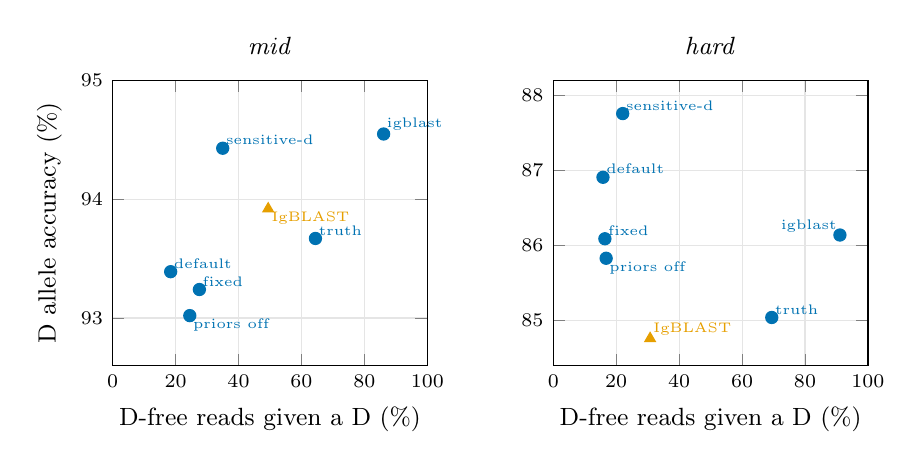
\begin{tikzpicture}
\begin{groupplot}[group style={group size=2 by 1,horizontal sep=1.6cm},
  width=0.46\linewidth,height=5.2cm,
  xlabel={D-free reads given a D (\%)},
  tick label style={font=\scriptsize},label style={font=\small},title style={font=\small},
  grid=major,grid style={gray!20},xmin=0,xmax=100,every axis plot/.append style={mark size=2.2pt},
  nodes near coords,point meta=explicit symbolic,
  every node near coord/.style={font=\tiny,anchor=south west,inner sep=1pt}]
\nextgroupplot[title={\emph{mid}},ylabel={D allele accuracy (\%)},ymin=92.6,ymax=95.0]
\addplot[only marks,mark=*,cSwig] coordinates {(18.44,93.39)[default] (27.57,93.24)[fixed] (34.98,94.43)[sensitive-d] (64.45,93.67)[truth] (86.12,94.55)[igblast]};
\addplot[only marks,mark=*,cSwig,every node near coord/.style={font=\tiny,anchor=north west,inner sep=1pt}] coordinates {(24.52,93.02)[priors off]};
\addplot[only marks,mark=triangle*,cIgb,every node near coord/.style={font=\tiny,anchor=north west,inner sep=1pt}] coordinates {(49.43,93.92)[IgBLAST]};
\nextgroupplot[title={\emph{hard}},ymin=84.4,ymax=88.2]
\addplot[only marks,mark=*,cSwig] coordinates {(15.79,86.91)[default] (16.4,86.09)[fixed] (22.06,87.76)[sensitive-d] (69.43,85.04)[truth]};
\addplot[only marks,mark=*,cSwig,every node near coord/.style={font=\tiny,anchor=north west,inner sep=1pt}] coordinates {(16.8,85.83)[priors off]};
\addplot[only marks,mark=*,cSwig,every node near coord/.style={font=\tiny,anchor=south east,inner sep=1pt}] coordinates {(91.09,86.14)[igblast]};
\addplot[only marks,mark=triangle*,cIgb] coordinates {(30.77,84.76)[IgBLAST]};
\end{groupplot}
\end{tikzpicture}
\caption{D accuracy against D-free specificity on IgSim reads. Circles are
\swig{} settings and calling profiles, the triangle is IgBLAST 1.22. A tool
can buy D accuracy by calling a D more often; better models lie up and to
the left.}
\label{fig:operating}
\end{figure}

\subsection{Where the remaining errors are}
\label{sec:errors}

\Cref{tab:derrors} attributes every wrong or missing D call on 10,000 IgSim
reads per preset to the step where it arose. With a remnant of at least 8
nucleotides, the true D is almost never outside the search windows (0.04\,\%
on \emph{hard}) and almost never covered by the called J or V, the failure
mode of sequential annotation. Most errors are adjudication errors: a
placement of a correct allele existed, but the path chose another allele.
These are short, mutated remnants that another allele explains as well or
better under the model. On remnants of 1--7 nucleotides about half of the errors are a declined D,
as the D prior intends for evidence this weak.

The same holds for V and J. Aligning every allele unbanded under the same
objective (an exhaustive oracle) found no V search error in 2,000 reads per
preset (from the same sample as \cref{tab:derrors}) and 1 and 3 J search
errors on \emph{mid} and \emph{hard}; the
remaining V errors are ties (26 and 84 reads) and model errors (12 and 68),
in which the exhaustive optimum itself is not the truth because mutations
fall on the positions that separate alleles.

\begin{table}[t]
\centering
\caption{Attribution of D errors (\% of reads with a D remnant in the class),
on a separate sample of 10,000 IgSim reads per preset (\cref{tab:igsim,tab:ablation,tab:calibration}
use another sample). ``Adjudication'': a placement of an
equivalent allele existed but the path took another D or none; ``not
found'': no such placement survived the D search.}
\label{tab:derrors}
\footnotesize
\begin{tabular}{@{}l rr rr@{}}
\toprule
 & \multicolumn{2}{c}{remnant $\ge 8$\,nt} & \multicolumn{2}{c}{remnant 1--7\,nt} \\
\cmidrule(lr){2-3}\cmidrule(l){4-5}
 & \emph{mid} & \emph{hard} & \emph{mid} & \emph{hard} \\
\midrule
reads                                      & 8,535 & 8,483 & 974 & 1,006 \\
D correct                                  & 97.90 & 91.76 & 51.85 & 44.83 \\
wrong D, adjudication                      & 1.91 & 6.90 & 17.25 & 16.60 \\
wrong D, not found                         & 0.12 & 0.83 & 5.34 & 6.76 \\
wrong D, outside the windows               & 0.00 & 0.04 & 0.00 & 0.00 \\
missing D, adjudication                    & 0.03 & 0.23 & 18.07 & 22.27 \\
missing D, not found                       & 0.04 & 0.26 & 7.50 & 9.54 \\
called J covers $\ge 3$ bases of the true D & 0.04 & 0.14 & 0.51 & 0.99 \\
\bottomrule
\end{tabular}
\end{table}

\subsection{Calibration}
\label{sec:calibration}

Posteriors are well calibrated wherever the candidates contain the truth
(\cref{fig:calibration}). The expected calibration error is at most 0.5\,\%
for V and 0.8\,\% for J on the \emph{easy}, \emph{mid} and \emph{hard}
presets, and 1.9\,\% for the D allele and
1.1\,\% for D presence on \emph{hard} (\cref{tab:calibration}). The D-allele
posterior is over-confident in the 0.5--0.95 range: reported probabilities
of 85\,\% correspond to 77--78\,\% observed. At 30\,\% SHM the V and J
posteriors are over-confident (ECE 9.8 and 13.2\,\%): when retrieval misses
the true gene, no candidate can carry its mass.

\begin{table}[t]
\centering
\caption{Calibration of the reported posteriors on IgSim reads: expected
calibration error (\%) and Brier score.}
\label{tab:calibration}
\footnotesize
\begin{tabular}{@{}l rrrr rrrr@{}}
\toprule
 & \multicolumn{4}{c}{ECE (\%)} & \multicolumn{4}{c}{Brier} \\
\cmidrule(lr){2-5}\cmidrule(l){6-9}
Preset & V & D & J & D presence & V & D & J & D presence \\
\midrule
easy       & 0.09 & 0.20 & 0.05 & 0.04 & 0.0004 & 0.0010 & 0.0006 & 0.0001 \\
mid        & 0.12 & 0.96 & 0.08 & 0.76 & 0.0064 & 0.0292 & 0.0063 & 0.0217 \\
hard       & 0.47 & 1.87 & 0.80 & 1.14 & 0.0278 & 0.0556 & 0.0343 & 0.0227 \\
30\,\% SHM & 9.78 & 20.91 & 13.22 & 2.53 & 0.1654 & 0.2340 & 0.1978 & 0.0488 \\
\bottomrule
\end{tabular}
\end{table}

\begin{figure}[t]
\centering
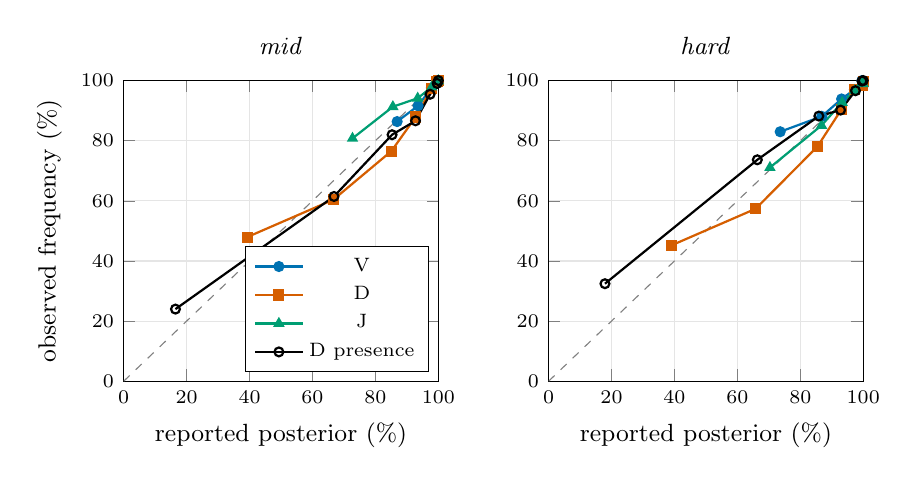
\begin{tikzpicture}
\begin{groupplot}[group style={group size=2 by 1,horizontal sep=1.4cm},
  width=0.46\linewidth,height=5.4cm,xmin=0,xmax=100,ymin=0,ymax=100,
  xlabel={reported posterior (\%)},
  tick label style={font=\scriptsize},label style={font=\small},title style={font=\small},
  grid=major,grid style={gray!20},every axis plot/.append style={mark size=1.6pt,line width=0.8pt},
  legend style={font=\scriptsize,at={(0.97,0.03)},anchor=south east}]
\nextgroupplot[title={\emph{mid}},ylabel={observed frequency (\%)}]
\addplot[gray,dashed,thin,forget plot] coordinates {(0,0) (100,100)};
\addplot[cV,mark=*] coordinates {(86.91,86.36) (93.56,91.61) (97.80,97.57) (99.69,99.78) (99.98,99.98)};
\addlegendentry{V}
\addplot[cD,mark=square*] coordinates {(39.24,47.93) (66.65,60.40) (85.08,76.54) (92.79,87.88) (97.87,97.42) (99.58,99.66) (99.98,99.90)};
\addlegendentry{D}
\addplot[cJ,mark=triangle*] coordinates {(72.72,80.77) (85.55,91.30) (93.44,94.12) (97.90,97.83) (99.67,99.60) (99.98,99.96)};
\addlegendentry{J}
\addplot[black,mark=o] coordinates {(16.46,23.99) (66.83,61.45) (85.30,81.99) (92.74,86.62) (97.38,95.45) (99.62,99.06) (100.00,99.99)};
\addlegendentry{D presence}
\nextgroupplot[title={\emph{hard}}]
\addplot[gray,dashed,thin,forget plot] coordinates {(0,0) (100,100)};
\addplot[cV,mark=*] coordinates {(73.61,82.98) (86.83,88.10) (93.13,93.88) (97.20,97.01) (99.59,100.00) (99.99,99.66)};
\addplot[cD,mark=square*] coordinates {(39.01,45.17) (65.79,57.35) (85.45,78.07) (93.08,90.41) (97.31,97.01) (99.62,98.37) (99.98,99.55)};
\addplot[cJ,mark=triangle*] coordinates {(70.35,71.07) (86.74,85.08) (93.29,92.72) (97.28,96.57) (99.57,99.19) (99.99,98.91)};
\addplot[black,mark=o] coordinates {(17.92,32.44) (66.34,73.65) (85.90,88.19) (92.80,90.18) (97.53,96.62) (99.59,99.85) (100.00,100.00)};
\end{groupplot}
\end{tikzpicture}
\caption{Reliability of the reported posteriors on IgSim reads: mean
reported probability against observed frequency of the event, per bin
(bins with at least 20 reads; most reads fall in the top bins). The event of
a segment is ``the reported names include the read's allele up to germline
equivalence'', that of D presence ``the read has a simulated D''.}
\label{fig:calibration}
\end{figure}

\subsection{Constant region}

On 10,000 IgSim reads per preset (both strands), about 80\,\% of which
continue into one of the 101 human IGHC alleles with a complete coding
start, the primary C call
is anchored-equivalent to the truth on 98.5--99.2\,\% of reads with 16--31
nucleotides of C and on at least 99.65\,\% from 32 nucleotides, and C was
called on at most 0.05\,\% of the about 2,000 reads per preset that stop
before C. C parts of 8--15 nucleotides are called on 53--60\,\% of reads, as
the 12-column floor intends. V, D and J calls are identical with and
without the C stage by construction.

\subsection{Speed}
\label{sec:speed}

\Cref{tab:speed} gives throughput on the 10,000-read IgSim sets, as wall
clock of the whole command, including database preparation (about 40\,ms
for the IMGT IGH set, every allele annotated on load). On four threads
\swig{} assigns 6,800--7,600 reads per second with posteriors, 76--88 times
IgBLAST's throughput on the same reads and machine, and 8,300--10,200 without
them; posteriors add 22--35\,\% to the run time. On the four out-of-sample
GenAIRR IGH sets (\cref{tab:oos}; machine lightly loaded) IgBLAST took
81--90\,s per 10,000 reads and \swig{} 1.0--1.4\,s. The SIMD kernel gives
2.5--2.7 times the throughput of the scalar kernel on one thread,
AVX-512BW's 32 lanes adding 2--7\,\% over AVX2's 16. Every backend and every
thread count produced byte-identical output on both sets.

\begin{table}[t]
\centering
\caption{Throughput on 10,000 IgSim reads (reads per second; wall clock of
the whole command including database preparation; median of three runs for
\swig). The default kernel on this CPU is AVX2: the default and AVX2
one-thread rows are the same configuration timed separately and differ by
run-to-run variation (about 5\,\%).}
\label{tab:speed}
\footnotesize
\begin{tabular}{@{}l rr@{}}
\toprule
Configuration & \emph{mid} & \emph{hard} \\
\midrule
\swig, 4 threads                          & 7,552  & 6,774 \\
\swig, 4 threads, no posteriors           & 10,211 & 8,272 \\
\swig, 1 thread                           & 1,986  & 2,053 \\
\swig, 1 thread, no posteriors            & 2,690  & 2,515 \\
\addlinespace
\swig, 1 thread, AVX-512BW (32 lanes)     & 2,235  & 2,188 \\
\swig, 1 thread, AVX2 (16 lanes)          & 2,089  & 2,152 \\
\swig, 1 thread, portable lanes (16)      & 1,575  & 1,612 \\
\swig, 1 thread, scalar kernel            & 842    & 877   \\
\addlinespace
IgBLAST 1.22, 4 threads                   & 85.5   & 89.6  \\
\bottomrule
\end{tabular}
\end{table}

% ===========================================================================
\section{Discussion}
\label{sec:discussion}

\swig{} replaces the sequence of local decisions of a conventional
annotator with one objective and its exact maximiser. Three consequences
stand out in the results. First, the failure mode that motivates joint
placement, a neighbouring segment absorbing a short D, has essentially
disappeared (\cref{tab:derrors}); the D errors that remain are choices
between similar alleles on short, mutated remnants, where the evidence is
present but weak. That is a modelling question, and the D trim and N/P
priors show that modelling, not search, is where further accuracy lies:
moving two cut-local prior terms into the graph raised IGH D accuracy on
GenAIRR reads by up to 3.1 points at no measurable cost in speed. Second,
because every non-alignment term is a log prior odds with a stated
derivation, the trade-off between finding short D remnants and leaving D-free
junctions alone has a single, interpretable knob, the prior odds of a D
(\cref{fig:operating}), rather than a set of thresholds. Third, the posterior
is a by-product of the same recursion and the call is its mode, so the
reported probabilities describe the call that is reported; they are well
calibrated up to IgG-like mutation levels.

The pair of simulators matters. GenAIRR scores calls against tie sets that
count only the bases a read actually shows, which rewards reporting genuine
ties and penalises over-reporting; IgSim scores germline equivalence and
separates D accuracy from D-free specificity and remnant length. On both,
the IgBLAST comparison favours \swig{} on V and D up to IgG-like mutation,
except D on IgM-like reads, where IgBLAST's lead comes from 1--3-nt remnants.
On IgSim, IgBLAST reports more exact junctions because \swig{} withholds a
junction whose anchor codon its alignments do not reach, and at 30\,\% SHM
IgBLAST's V calls are better.

\subsection{Limitations}

\begin{itemize}
  \item \emph{All results are on simulated reads.} Both simulators make
    simplifying assumptions: uniform allele usage, independent trims, no
    chimeras or long adapters, and in IgSim no hotspot-targeted SHM and no
    codon-length indels. Several design parameters were measured on
    simulated reads: the open-flank allowance from simulated junction
    lengths, the D-cost credit on IgSim, and the D trim and N/P priors from
    an analysis of the previous release's losses on the GenAIRR sets of
    \cref{tab:genairr}. The priors' means (5, 7 and 8 bases) are generic
    rather than fitted, and GenAIRR's own trim tables did no better in the
    prototype; on GenAIRR reads disjoint from the design sets the priors
    gained as much (\cref{tab:oos}), but both come from one simulator.
    Validation on real repertoires, for example donors with sequenced
    germline genotypes, is the most important next step.
  \item \emph{Comparisons.} We did not compare with partis, IMGT/V-QUEST
    or MiXCR~4 (which requires a licence key).
  \item \emph{The plausibility constraints are inherited thresholds}, not
    terms of the likelihood, and the call under them is the best admissible
    subset optimum rather than an exact maximum over every admissible path.
    They cost 0.4--2.9 points of junction exactness on simulated reads
    (\cref{tab:ablation}) in exchange for robustness on truncated, chimeric
    and cross-locus reads that the simulators do not produce. A model of
    truncation and template switching would price what they forbid.
  \item \emph{D on D-free junctions.} 16--18\,\% of IgSim reads without a D
    remnant still receive one, and a chance D within about 30 bases of a
    truncated read's V is indistinguishable from a real D there
    (\cref{tab:truncated}). On TRB, whose two D genes are short and rarely
    trimmed as much as the prior expects, the D-cost credit gives D-free
    reads a D more often.
  \item \emph{Extreme mutation.} At 30\,\% SHM the strand test and seed
    retrieval lose intact $k$-mers: 4.4\,\% of reads are left uncalled, 3.5\,\%
    because the wrong strand was chosen, V accuracy falls below IgBLAST's, and
    the V and J posteriors are
    over-confident because the true gene is no longer among the candidates.
  \item \emph{Statistics.} E-values use exact ungapped $\lambda$ and $K$
    (anti-conservative for gapped scores) and the total database length
    (conservative for near-identical alleles); they gate hits and are not
    calibrated $p$-values. One divergence per read assumes uniform mutation
    across V, D and J.
  \item \emph{One alignment per D allele and window.} A D allele's optimal
    local alignment in its window need not be its best clip at the chosen
    cuts; this is the one remaining approximation of the segmentation model.
\end{itemize}

\subsection{Future work}

The D-presence residual of the posterior tracks junction length, which
points to an N/P length prior that decides D presence and not only re-ranks
Ds. Allele usage is uniform in the model; usage priors learned from the
repertoire itself, iterated with the calls, would matter where one gene
dominates. Gapped Karlin--Altschul parameters and an effective database size
can be fitted by simulation. Above all, the model's assumptions need testing
on real data.

\section{Conclusion}

\swig{} shows that germline assignment can be posed as one likelihood ratio
and solved exactly, fast enough for whole repertoires: an exact semi-Markov
recursion over every pair of cuts between neighbouring segments, priors
derived as prior odds over the hypotheses each segment competes with, calls
valued at each read's own divergence and posteriors from the same recursion.
Every search shortcut carries a stated guarantee, and the remaining errors
are located by construction. On GenAIRR reads it is the most accurate of the
tools compared on V, D and J on every immunoglobulin set and on D for TRB,
including on reads disjoint from those its D priors were designed on; on
IgSim reads it leads IgBLAST on V and D up to IgG-like mutation (except
IgM-like D, where IgBLAST's lead comes from unidentifiable 1--3-nt remnants)
and trails on junction exactness and on V at 30\,\% SHM. It runs nearly two
orders of magnitude faster than IgBLAST.

\section*{Availability}

\swig{} 0.39.7 is free software under the MIT licence, available at
\url{https://github.com/mashu/swig} (Rust crate in \code{engine/}). It builds
with \code{cargo build -{}-release} on Rust $\ge 1.89$, has no dependencies,
and runs on x86-64 and AArch64 and as WebAssembly. The command
\code{swig -{}-v V.fasta -{}-d D.fasta -{}-j J.fasta reads.fastq} writes AIRR
Rearrangement TSV; \code{swig simulate} and \code{swig evaluate} reproduce
the IgSim evaluation for any germline set and any tool's AIRR output. The
scripts and settings that produce every \swig{} and IgBLAST number in this
paper are distributed with the source.


\section*{Acknowledgements}

% TODO: acknowledgements and funding.
To be added.

\bibliographystyle{unsrtnat}
\bibliography{references}

\end{document}
